
\subsection{Term unfolding for homogeneous inputs}
\label{sec:homo-unfold}



\subsubsection{Term unfolding for $\alpha$-homogeneous inputs}
\label{subsec:alpha-homo-unfold}

For a monotone function 
\begin{align*}
\alpha: \set{1,\ldots,k} \to \set{1,\ldots,k}
\end{align*}
we say that a term $ t \in \tmonad \mati k \rSigma$ is $\alpha$-homogeneous if all internal branches have twist $\alpha$. This section is devoted to proving the following lemma. 

\begin{lemma}\label{lem:homo-twist}
    Let $k \in \set{1,2,\ldots}$ and let $\alpha : \set{1,\ldots,k} \to \set{1,\ldots,k}$ be a monotone function. There is a derivable operation 
    \begin{align*}
        \ranked{f : \tmonad \mati k \rSigma \to \mati k {(\tmonad \Sigma)} }
        \end{align*}      
which coincides with term unfolding for all inputs which are $\alpha$-homogeneous.
\end{lemma}

\begin{proof}
We proceed by induction on $k$. When $k=1$, the unfolding coincides with the basic distributivity function 
\begin{align*}
\ranked{ \tmonad \reduce 1 \Sigma \to {\reduce 1 \tmonad \Sigma}}
\end{align*}
Let us treat the inductive case. For that, we introduce a tool that will be useful to analyze the function $\alpha$. For a function $$\alpha: \set{1,\ldots,k} \to \set{1,\ldots,k}$$ define  \emph{its graph} as the directed graph whose set of vertices is $\set{1,\ldots,k}$, and which contains an edge $i\rightarrow j$ if $\alpha(i)=j$. Note that the out-degree of the nodes is $1.$

\medskip
In the proof of the inductive case, we distinguish two cases. The first one is when the graph of $\alpha$ is not weakly connected. In this case, by monotonicity of $\alpha$, we can find $m\in \set{1,k-1}$ such that $\alpha(\set{1,m})\subseteq\set{1,m}$ and $\alpha(\set{m+1,k})\subseteq\set{m+1,k}$. The idea is then to create two copies of the original tree: in the first one we keep only the first $m$ elements of the tensor product of each node, and in the second one we keep the last $k-m$ copies. Then we unfold these terms by applying the induction hypothesis, and  finally we gather them to obtain the  unfolding of the original term. 

%\smallskip
%To illustrate this case, we consider the following function $\alpha$, whose graph is shown below
%\begin{center}
%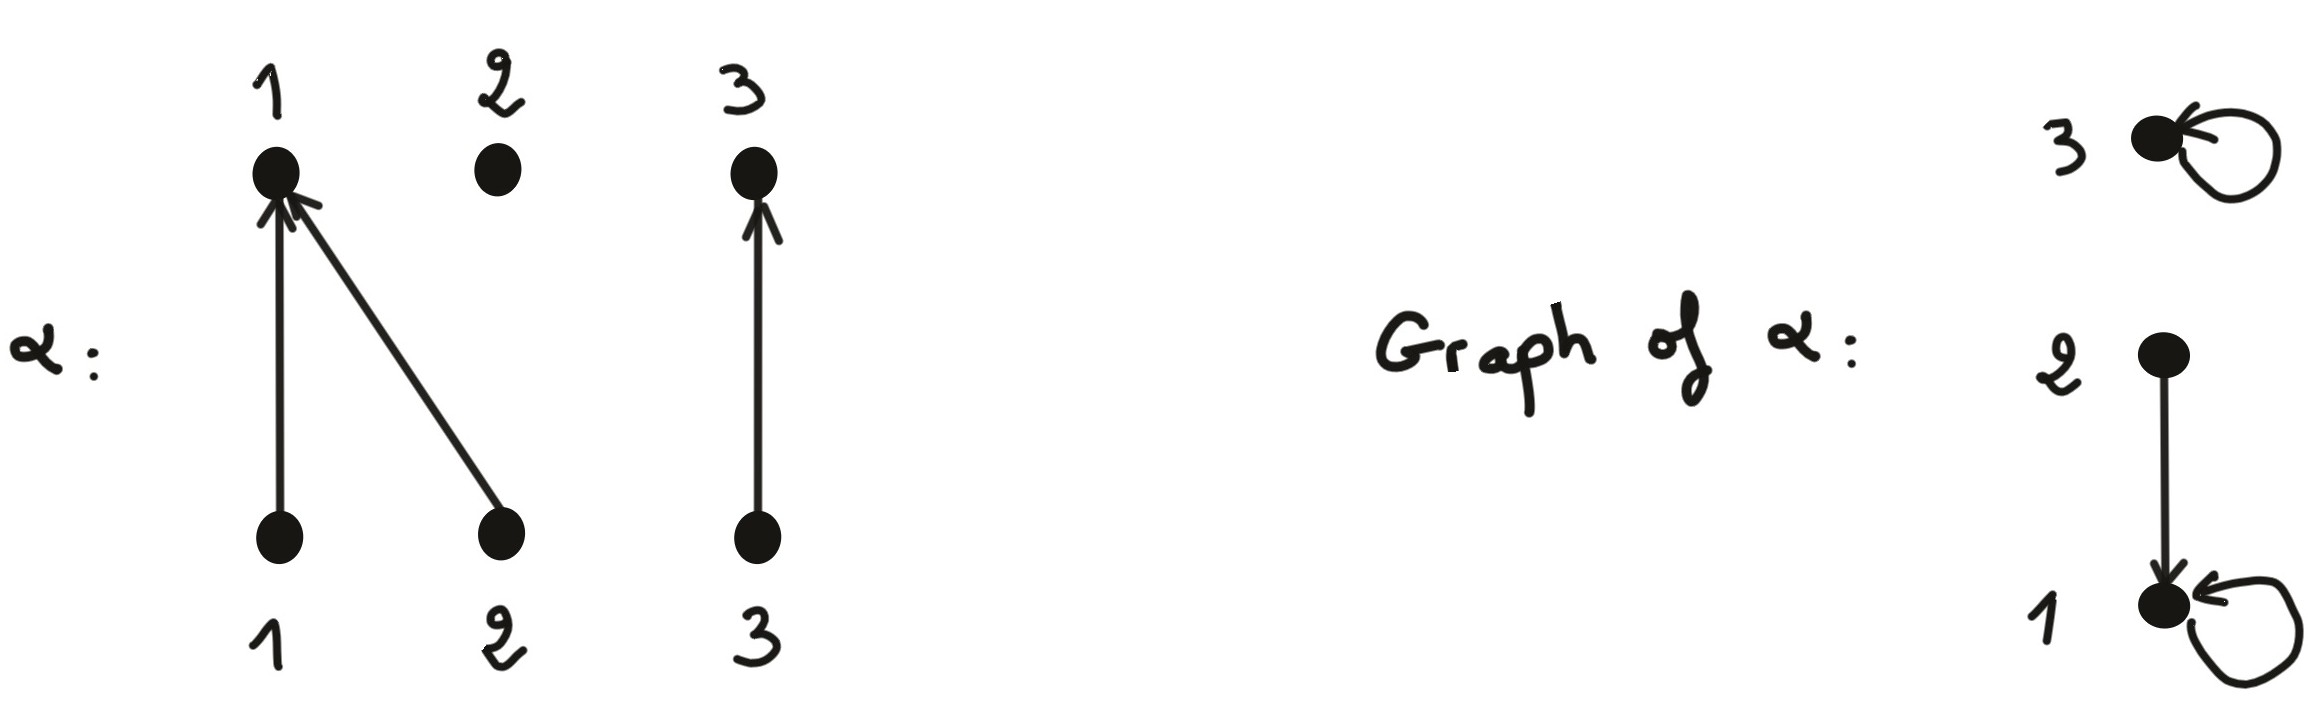
\includegraphics[scale=.07]{MyPic27.jpg}
%\end{center}
%The graph of $\alpha$ is not weakly connected: it contains two weakly connected components, $\set{1,2}$ and $\set{3}$.
%Consider the following $\alpha$-homogeneous terms $t$ of $\tmonad \mati k \rSigma$ which will be our running example in the not weakly connected case of the proof. We colored in blue the elements of the first weakly connected part of the graph of $\alpha$ and in green the second part.
%\begin{center}
%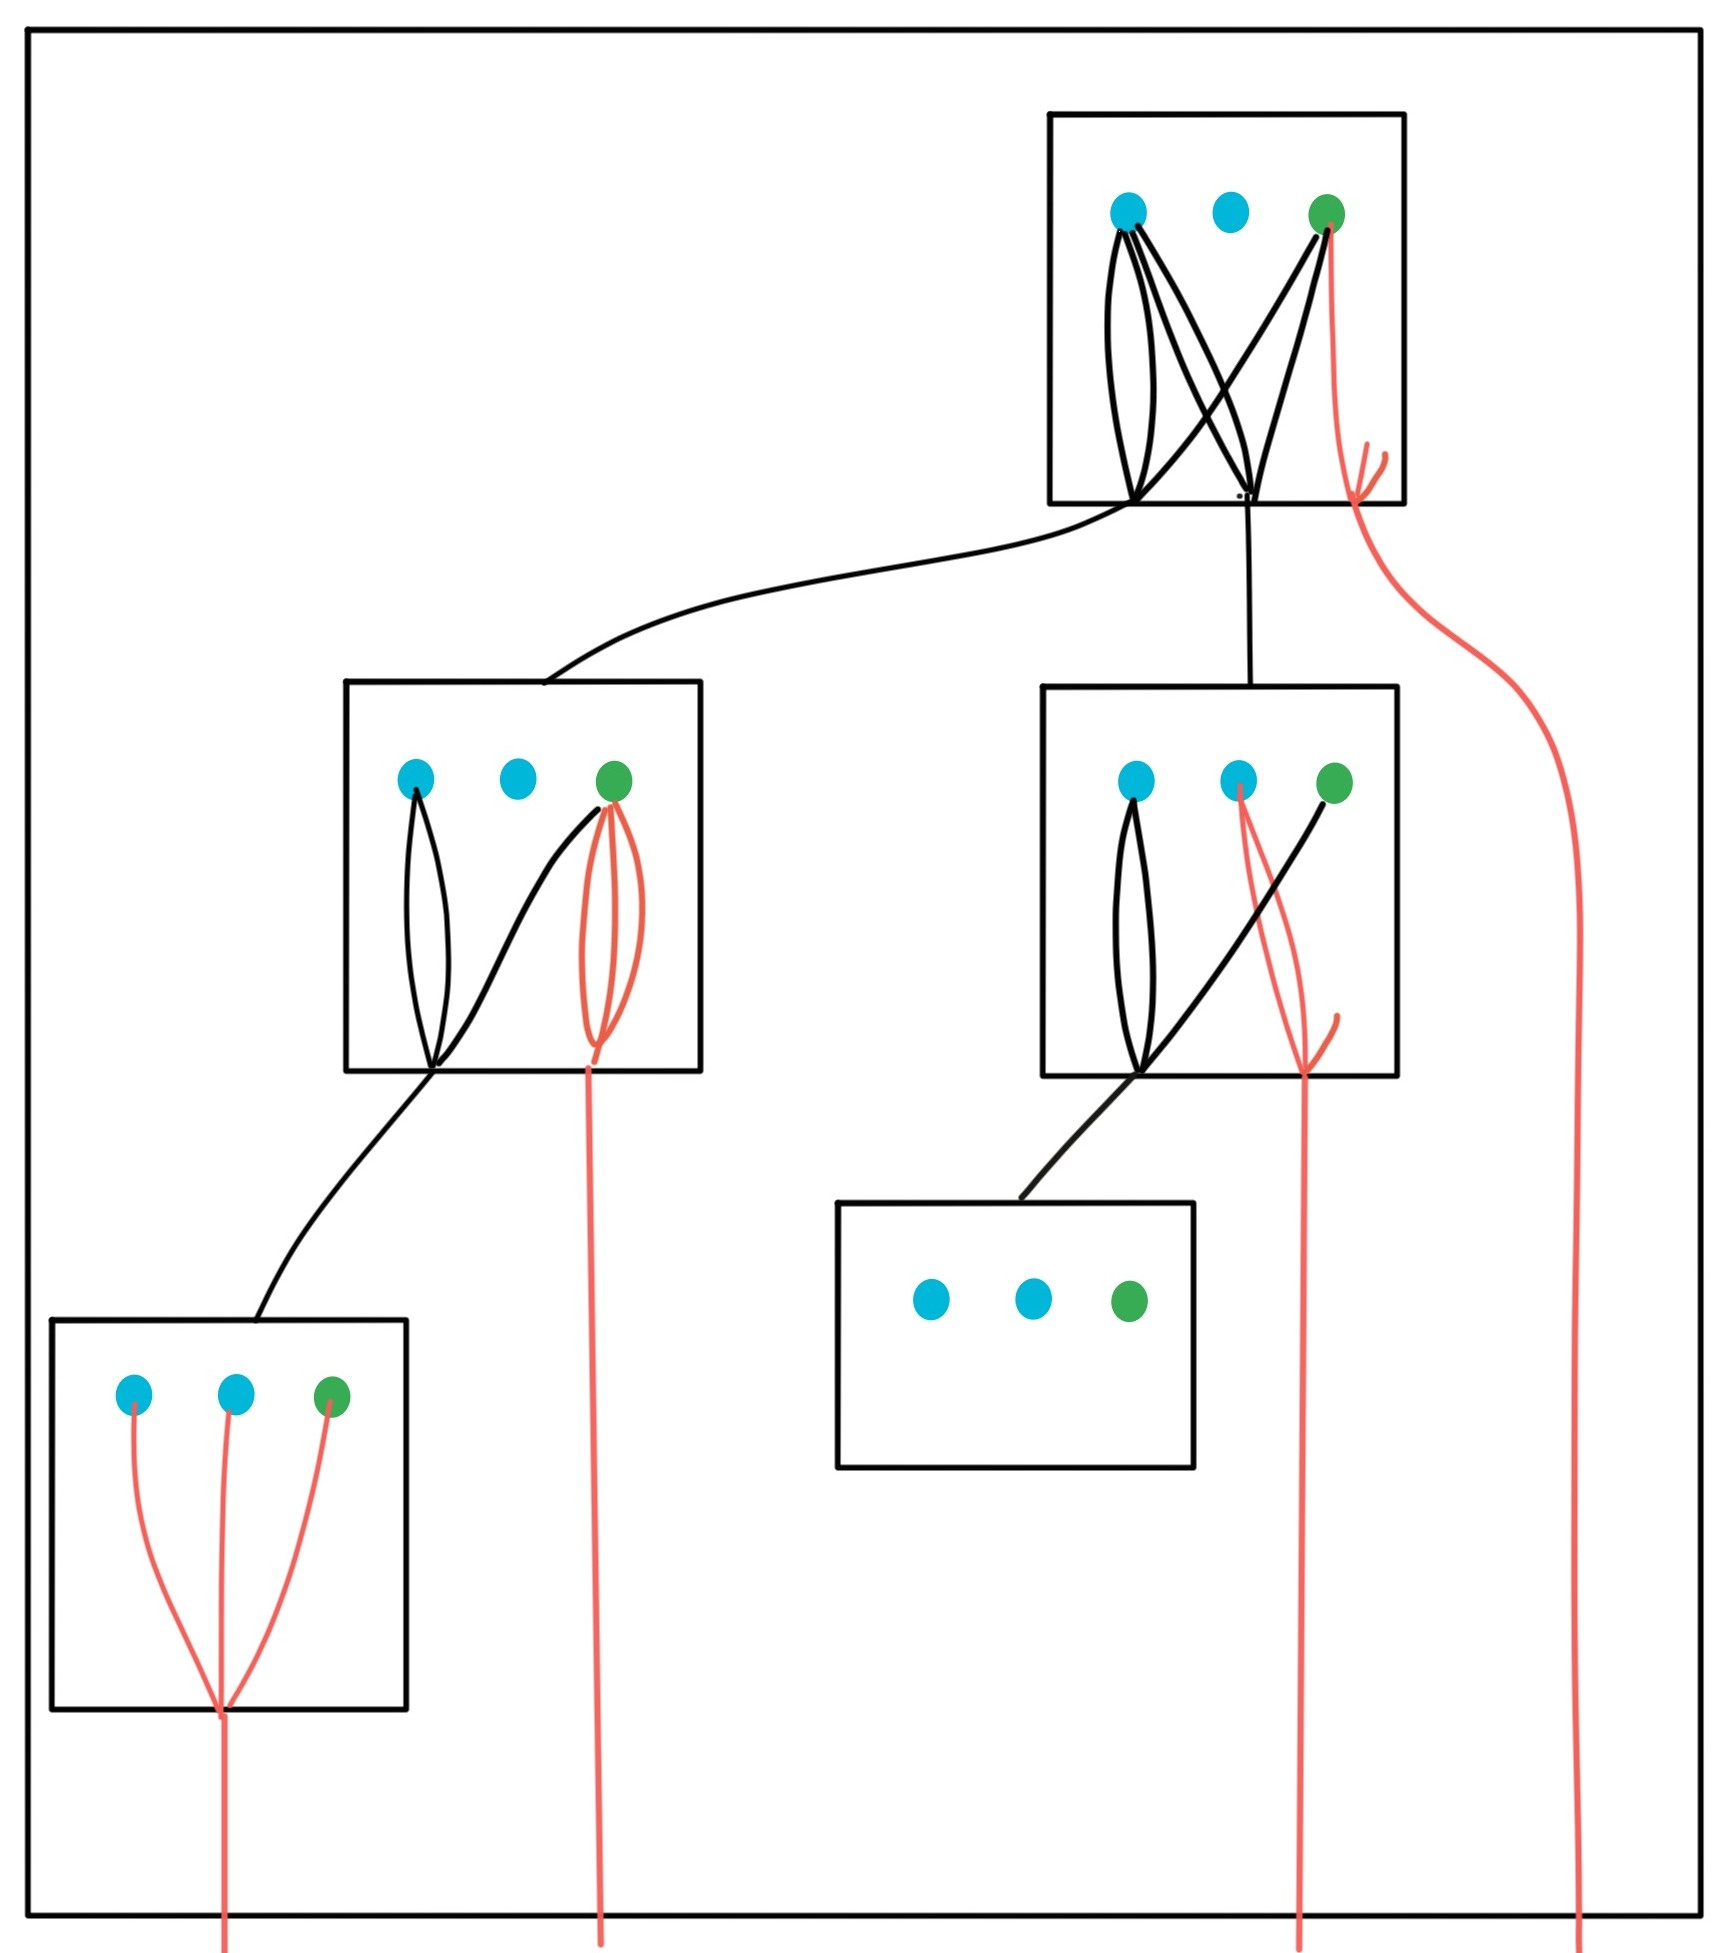
\includegraphics[scale=.07]{MyPic28.jpg}
%\end{center}
Let us now implement the ideas we discussed above. We start by unfolding the external twists, using the basic external unfold function. This way, the domain of every external twist  cannot be shared by the two disconnected components of the domain of $\alpha$.
%Our running example becomes like this:
%\begin{center}
%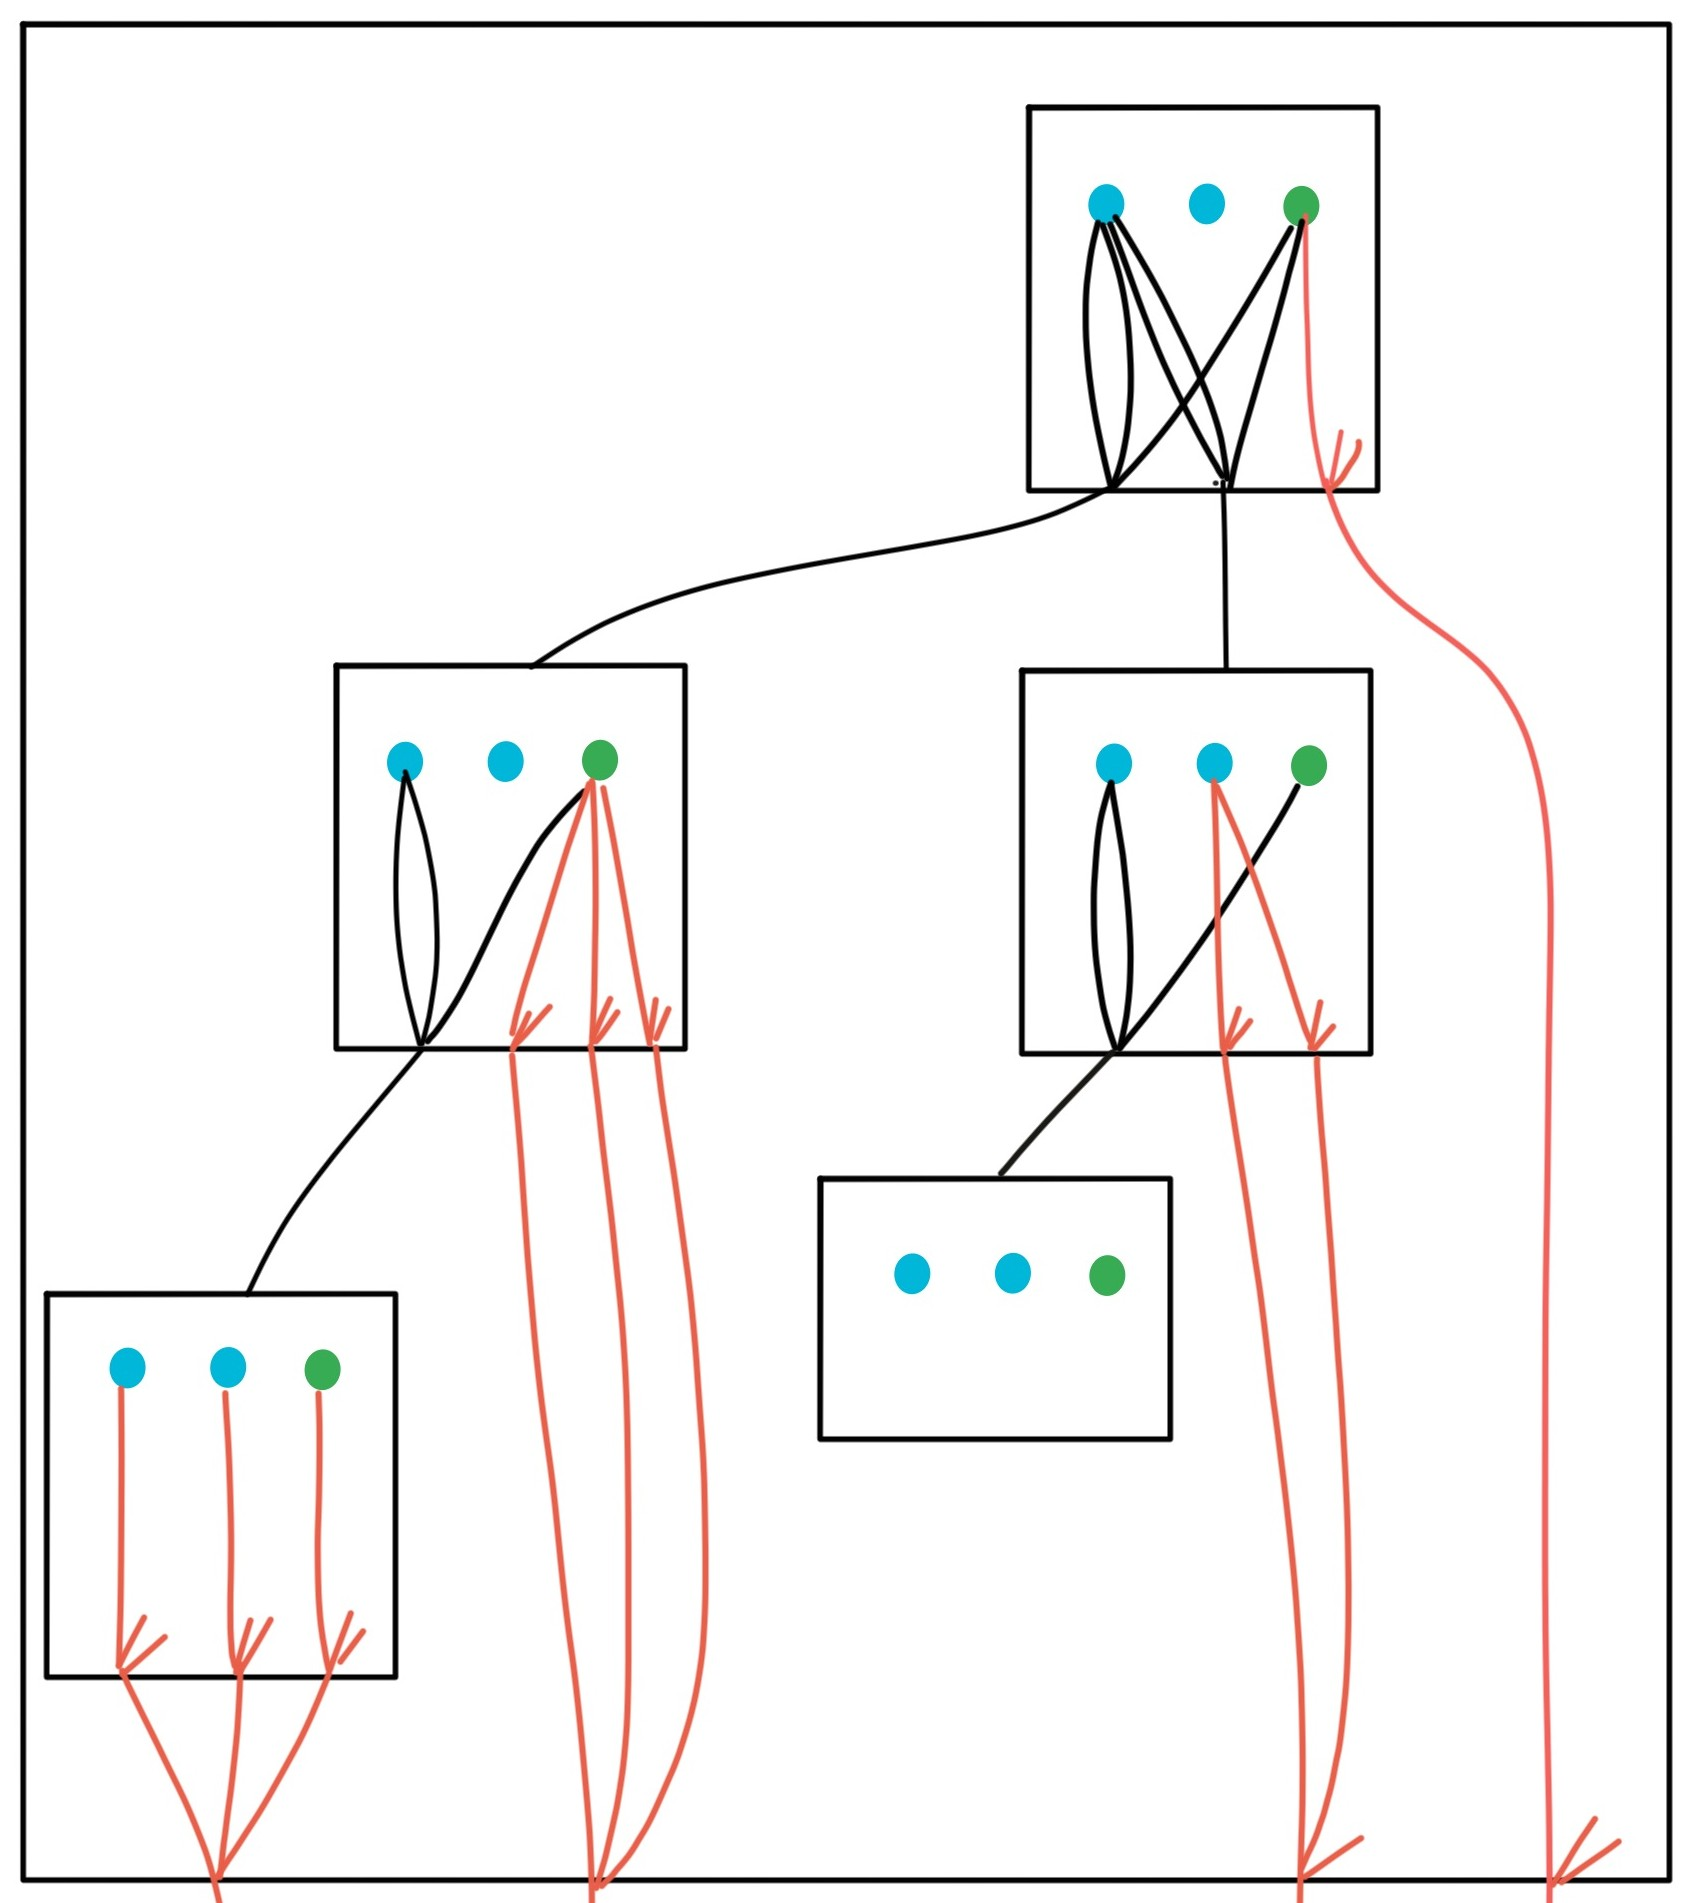
\includegraphics[scale=.07]{MyPic29.jpg}
%\end{center}
Then, we duplicate the input term using the basic function 
\begin{align*}
\ranked{\tmonad \mati k \Sigma\to \reduce 2 (\tmonad \mati k \Sigma\otimes \tmonad \mati k \Sigma)}
\end{align*}
To the first copy, we apply the function  
\begin{align*}
\ranked{f_1:\tmonad \mati k \Sigma \to \mati m {(\tmonad \Sigma)}}
\end{align*}
which keeps only the first $m$ elements of the tensor product, then applies the induction hypothesis to the obtained term.
To the second copy, we apply the function 
\begin{align*}
\ranked{f_2:\tmonad \mati k \Sigma \to \mati {k-m} {(\tmonad \Sigma)}}
\end{align*}
which keeps only the last $k-m$ elements of the tensor product, then applies the induction hypothesis to the obtained term.

%Here is the effect of the functions $f_1$ and $f_2$ on our example
%\begin{center}
%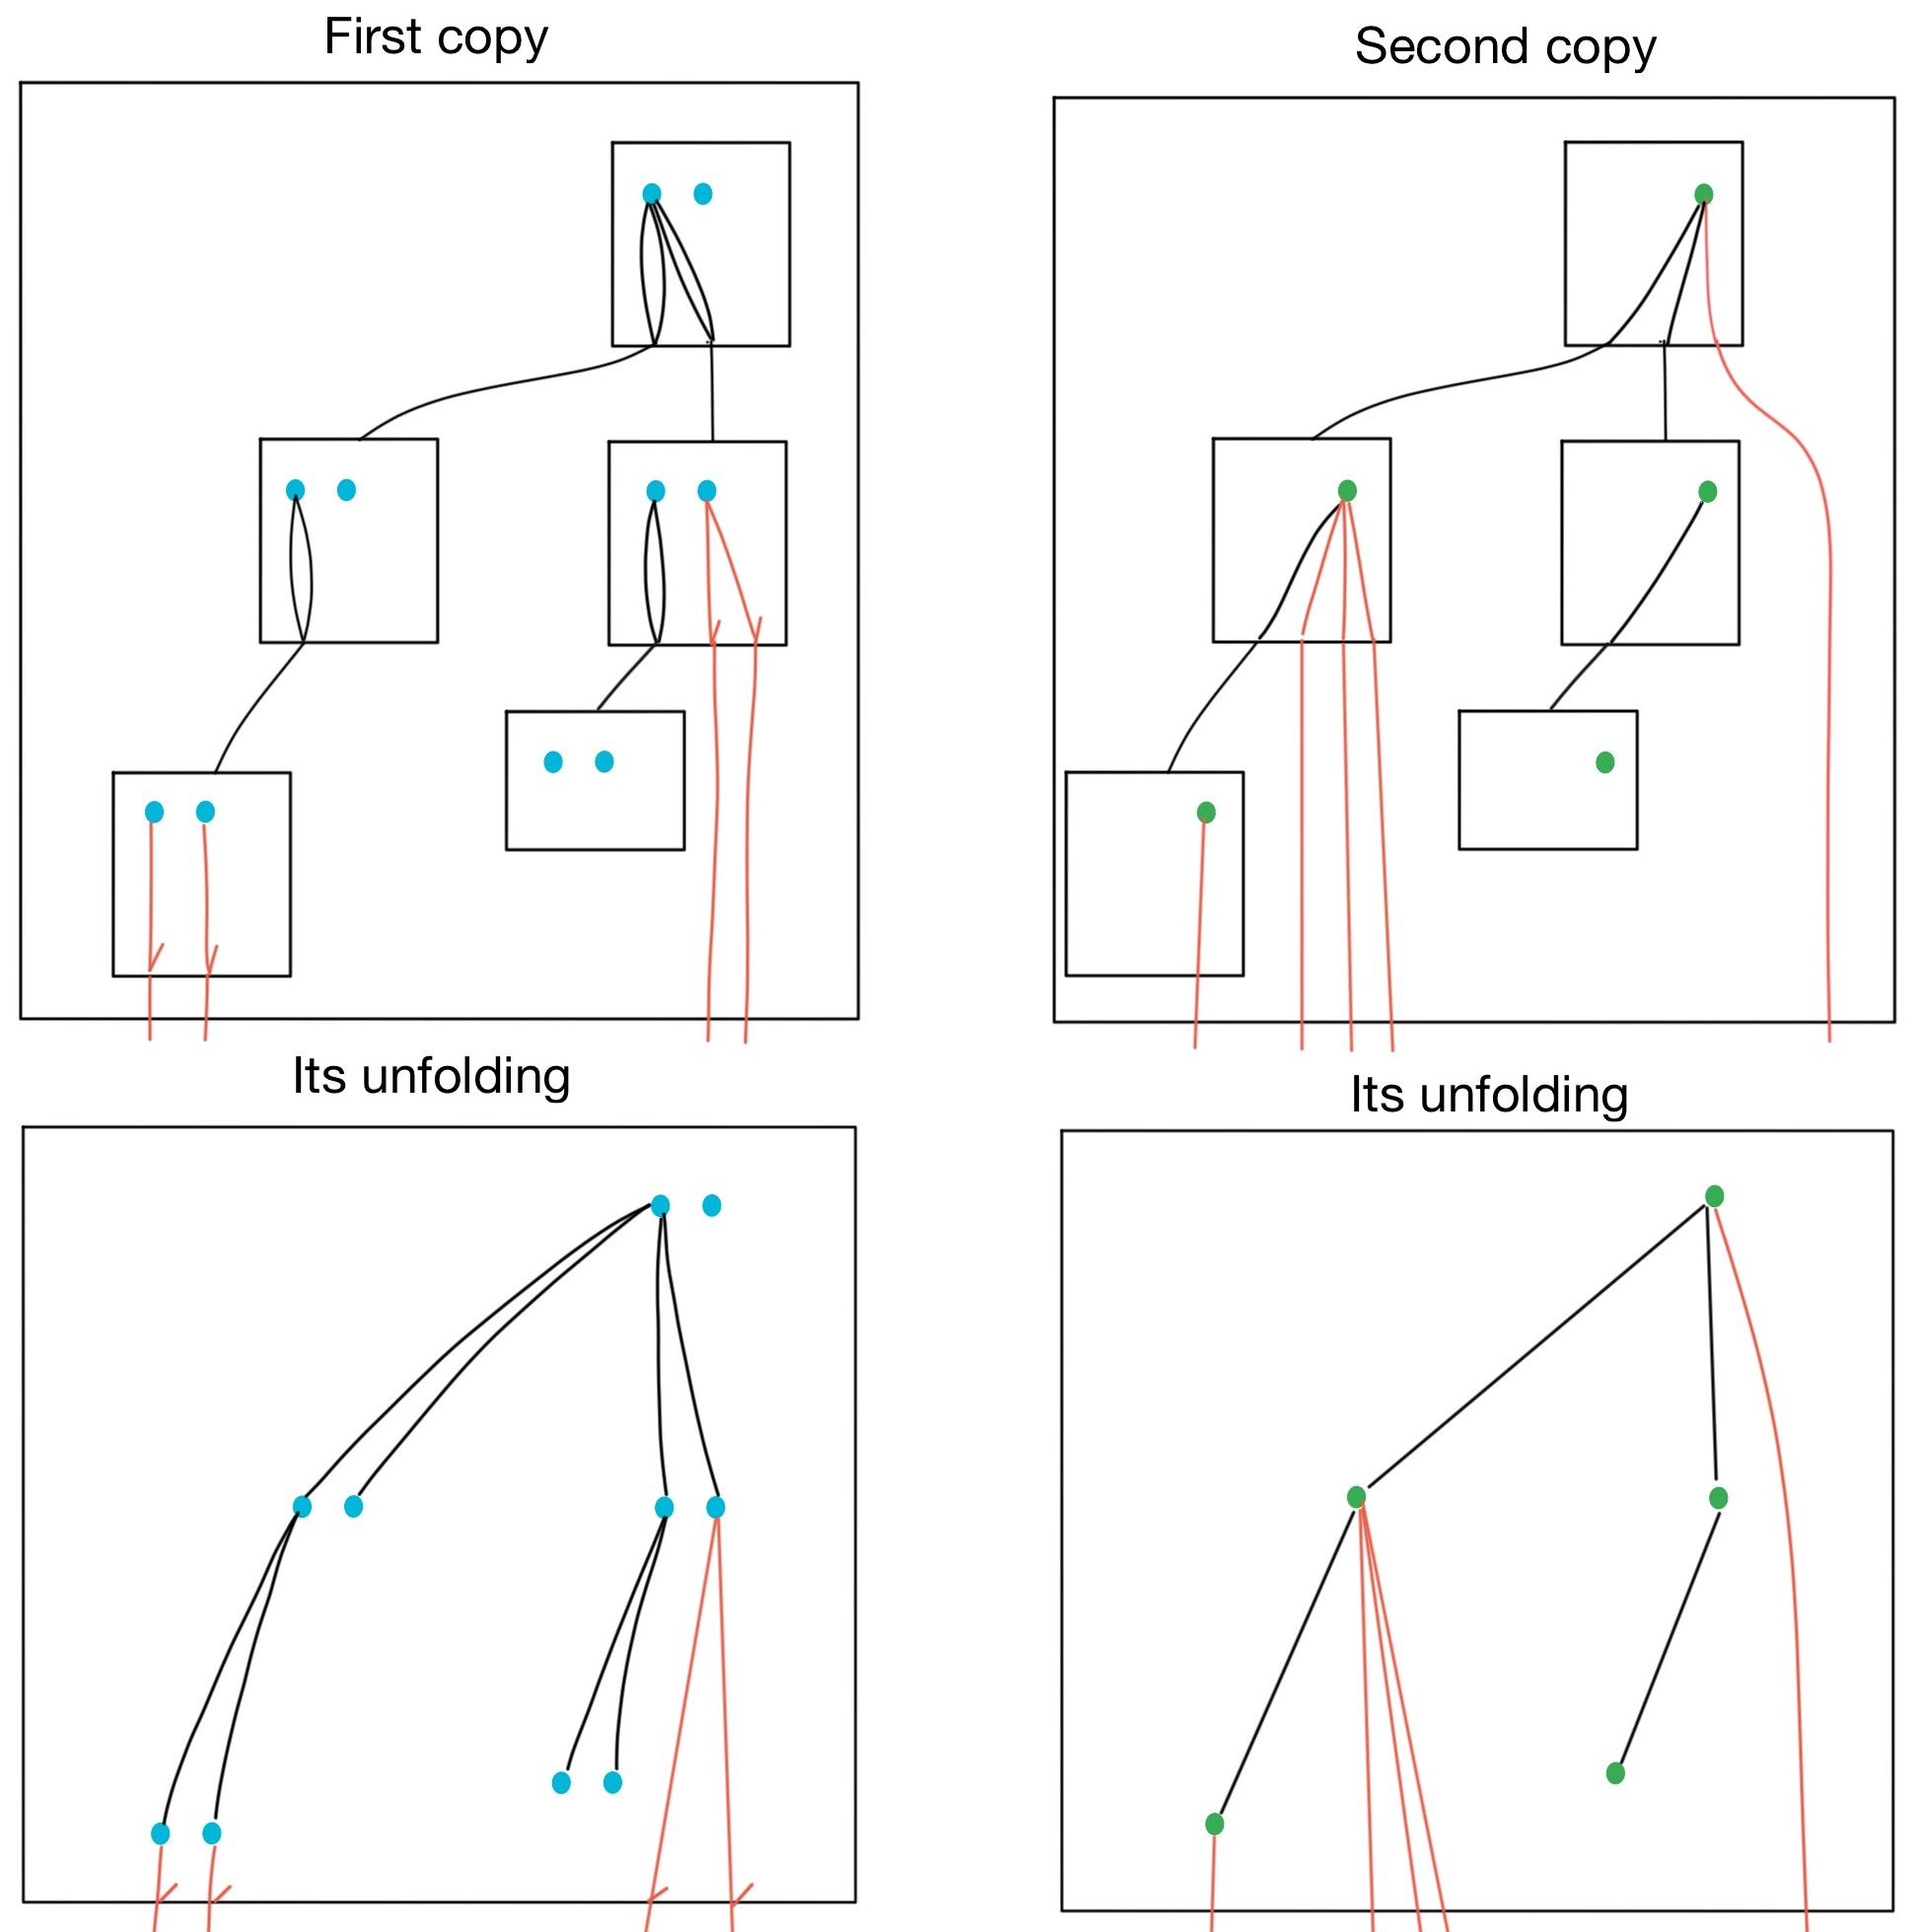
\includegraphics[scale=.15]{MyPic30.jpg}
%\end{center}
 The function $\ranked{f_1}$ can be derived using the tensor projection function, the merge of folds, then reducing the fold and finally invoking the induction hypothesis. 
%\begin{align*}
%\begin{prooftree}
%\Hypo{\overbrace{\ranked{\mati k \Sigma \to \reduce k \reduce 1 \Sigma^m}}^{\substack{\text{Lift the projection on the first}\\\text{$m$ elements of the tensor to $\reduce k$}}}}
%\Hypo{\overbrace{\ranked{\reduce k \reduccomponenetse 1 \Sigma^m \to \reduce k \Sigma^m}}^{\substack{\text{Merge the folds $\reduce k$ and $\reduce 1$}}}}
%\Hypo{\overbrace{\ranked{\reduce k \Sigma^m \to \mati m {(\Sigma\cdot (1+0))}}}^{\substack{\text{Adjust the degree of the fold}\\\text{to get a matrix power}}}}
%\Infer{3}[]{\ranked{\mati k \Sigma \to \mati m {(\Sigma\cdot (1+0))}}}
%\end{prooftree}
%\end{align*}


When we apply $f_1$ and $f_2$ to the two copies of the original term, we get a term of type 
\begin{align*}
\ranked{ \reduce 2 (\mati m {(\tmonad \Sigma)}\otimes  \mati {k-m} {(\tmonad\Sigma)})}
\end{align*}
%Now, we need to get the fold outside the tensor product. For that, we lift both $\ranked{\mati m {(\tmonad \Sigma)}}$ and $\ranked{\mati {k-m} {(\tmonad \Sigma)}}$ to $\ranked{\reduce k (\tmonad \Sigma)^m}$ and $\ranked{\reduce k (\tmonad \Sigma)^{k-m}}$ respectively. Then we commute the fold with the tensor product using the following basic function:
%\begin{align*}
%\ranked{\reduce k (\tmonad \Sigma)^m\otimes\reduce k (\tmonad \Sigma)^{k-m}\to \reduce k (\tmonad \Sigma)^k}
%\end{align*}
%Then we merge the two  folds $\reduce 2$ and $\reduce k$ into $\reduce {2k}$. After these operations, we get the desired term, but not with the desired type (the type we get is $\ranked{\reduce {2k} (\tmonad\Sigma)^k}$). To get the right type, which is $\ranked{\mati k {(\tmonad\Sigma)}}$, we apply the  function which reduces the degree of the fold
%\begin{align*}
%\ranked{\reduce {2k} (\tmonad \Sigma)^k \to \reduce {k} (\tmonad \Sigma)^k}
% \end{align*}
% The term we get for our example is the following, which is the unfolding of the original term
% \begin{center}
% 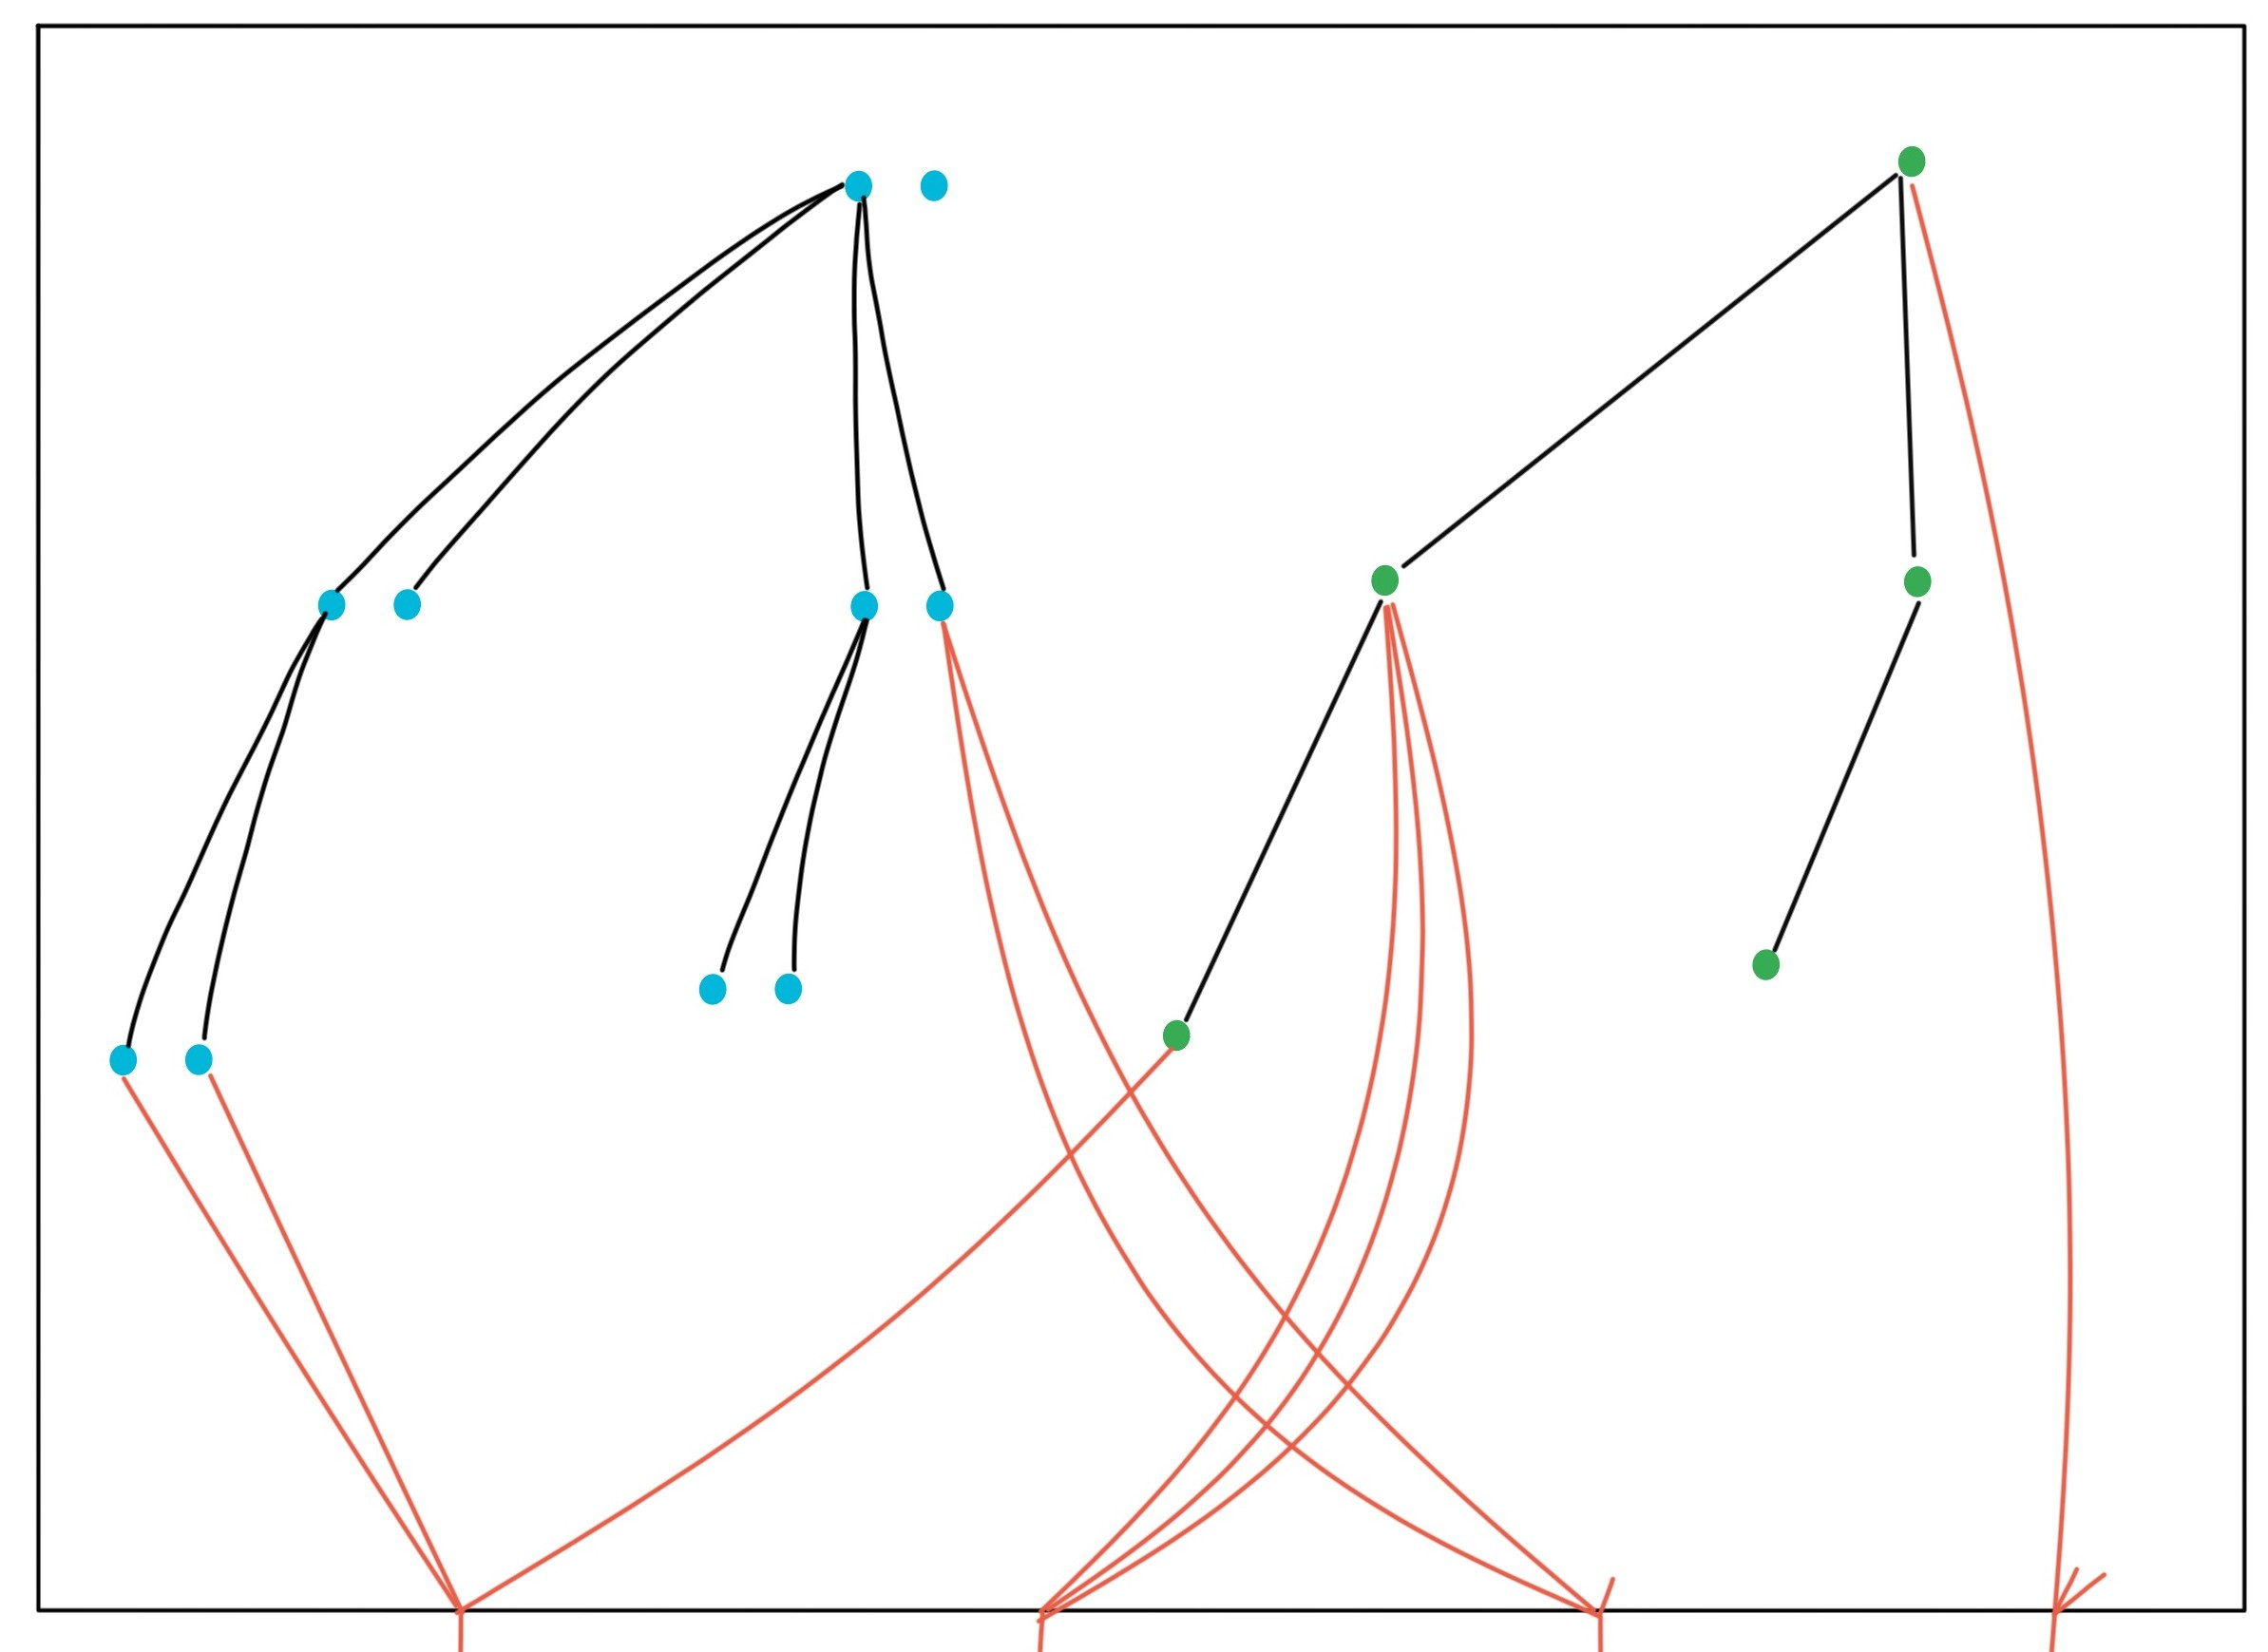
\includegraphics[scale=.08]{MyPic31.jpg}
% \end{center}
Apres une serie dinjections, de distributivites et de reductions de fold on obtien le resultat. Ptit truc: lorsqu'on reduit les fold, on a un bottom, qu'on fait remonter a la surface en utilisant une fonction d'error raising, a la fin on s'en debarasse dans le type en plongeant $\bot$ dans un arbre si on suppose que notre signature contient un element zeroaire et un element bianire. 
\medskip

Now consider the case where the graph of $\alpha$ is weakly connected. By monotonicity, we can show that either
\begin{align*}
\alpha^{-1}(1)=\emptyset\qquad\text{ or }\qquad\alpha^{-1}(k)=\emptyset
\end{align*}
By symmetry, we suppose wlog that $\alpha^{-1}(k)=\emptyset$. We suppose also that $\alpha(k)=k-1$, the general case can be treated in a similar way.
We consider as example the following function $\alpha$, whose graph, drawn below, is weakly connected
\begin{center}
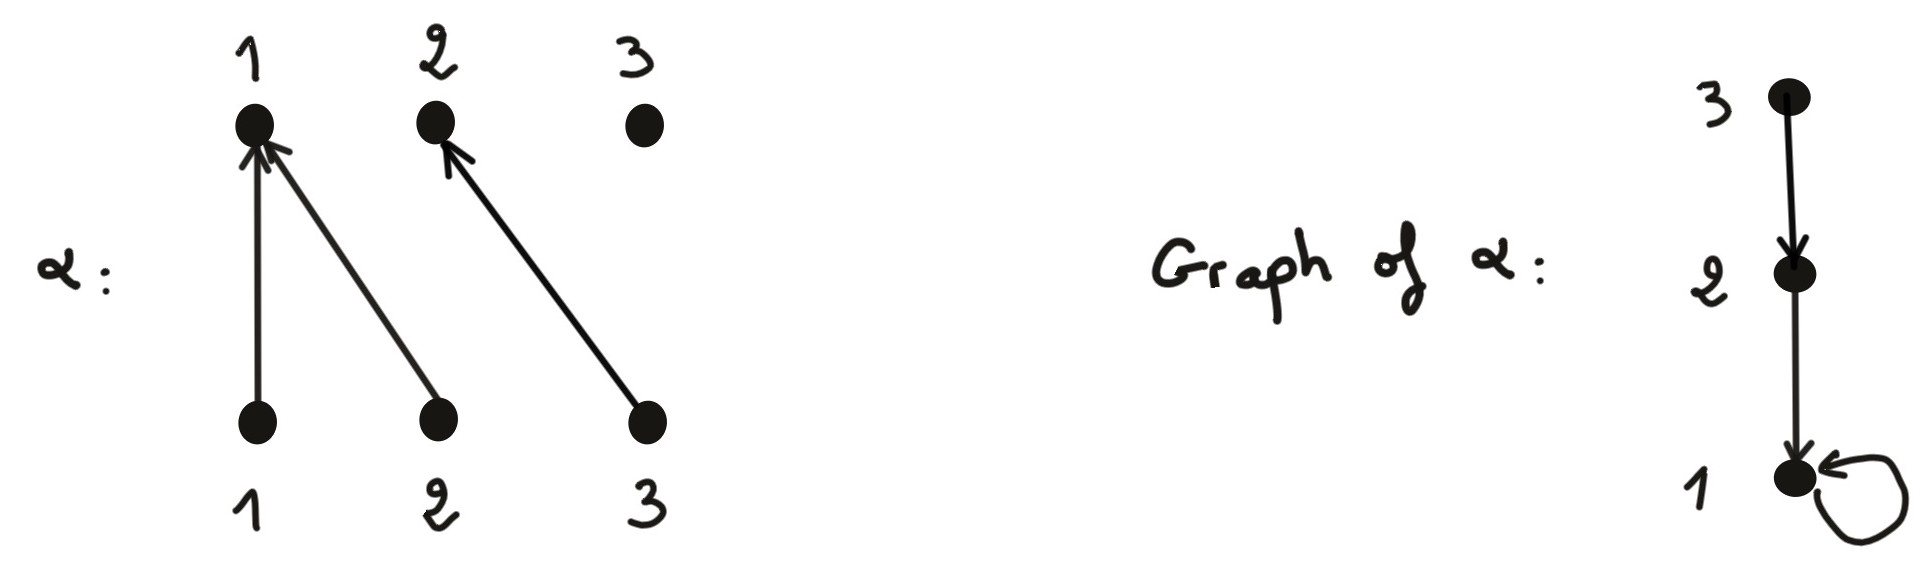
\includegraphics[scale=.1]{MyPic32.jpg}
\end{center}
we consider also the following $\alpha$-homogeneous term, where $\alpha$ is the function above, as running example for the weakly connected case. 
\begin{center}
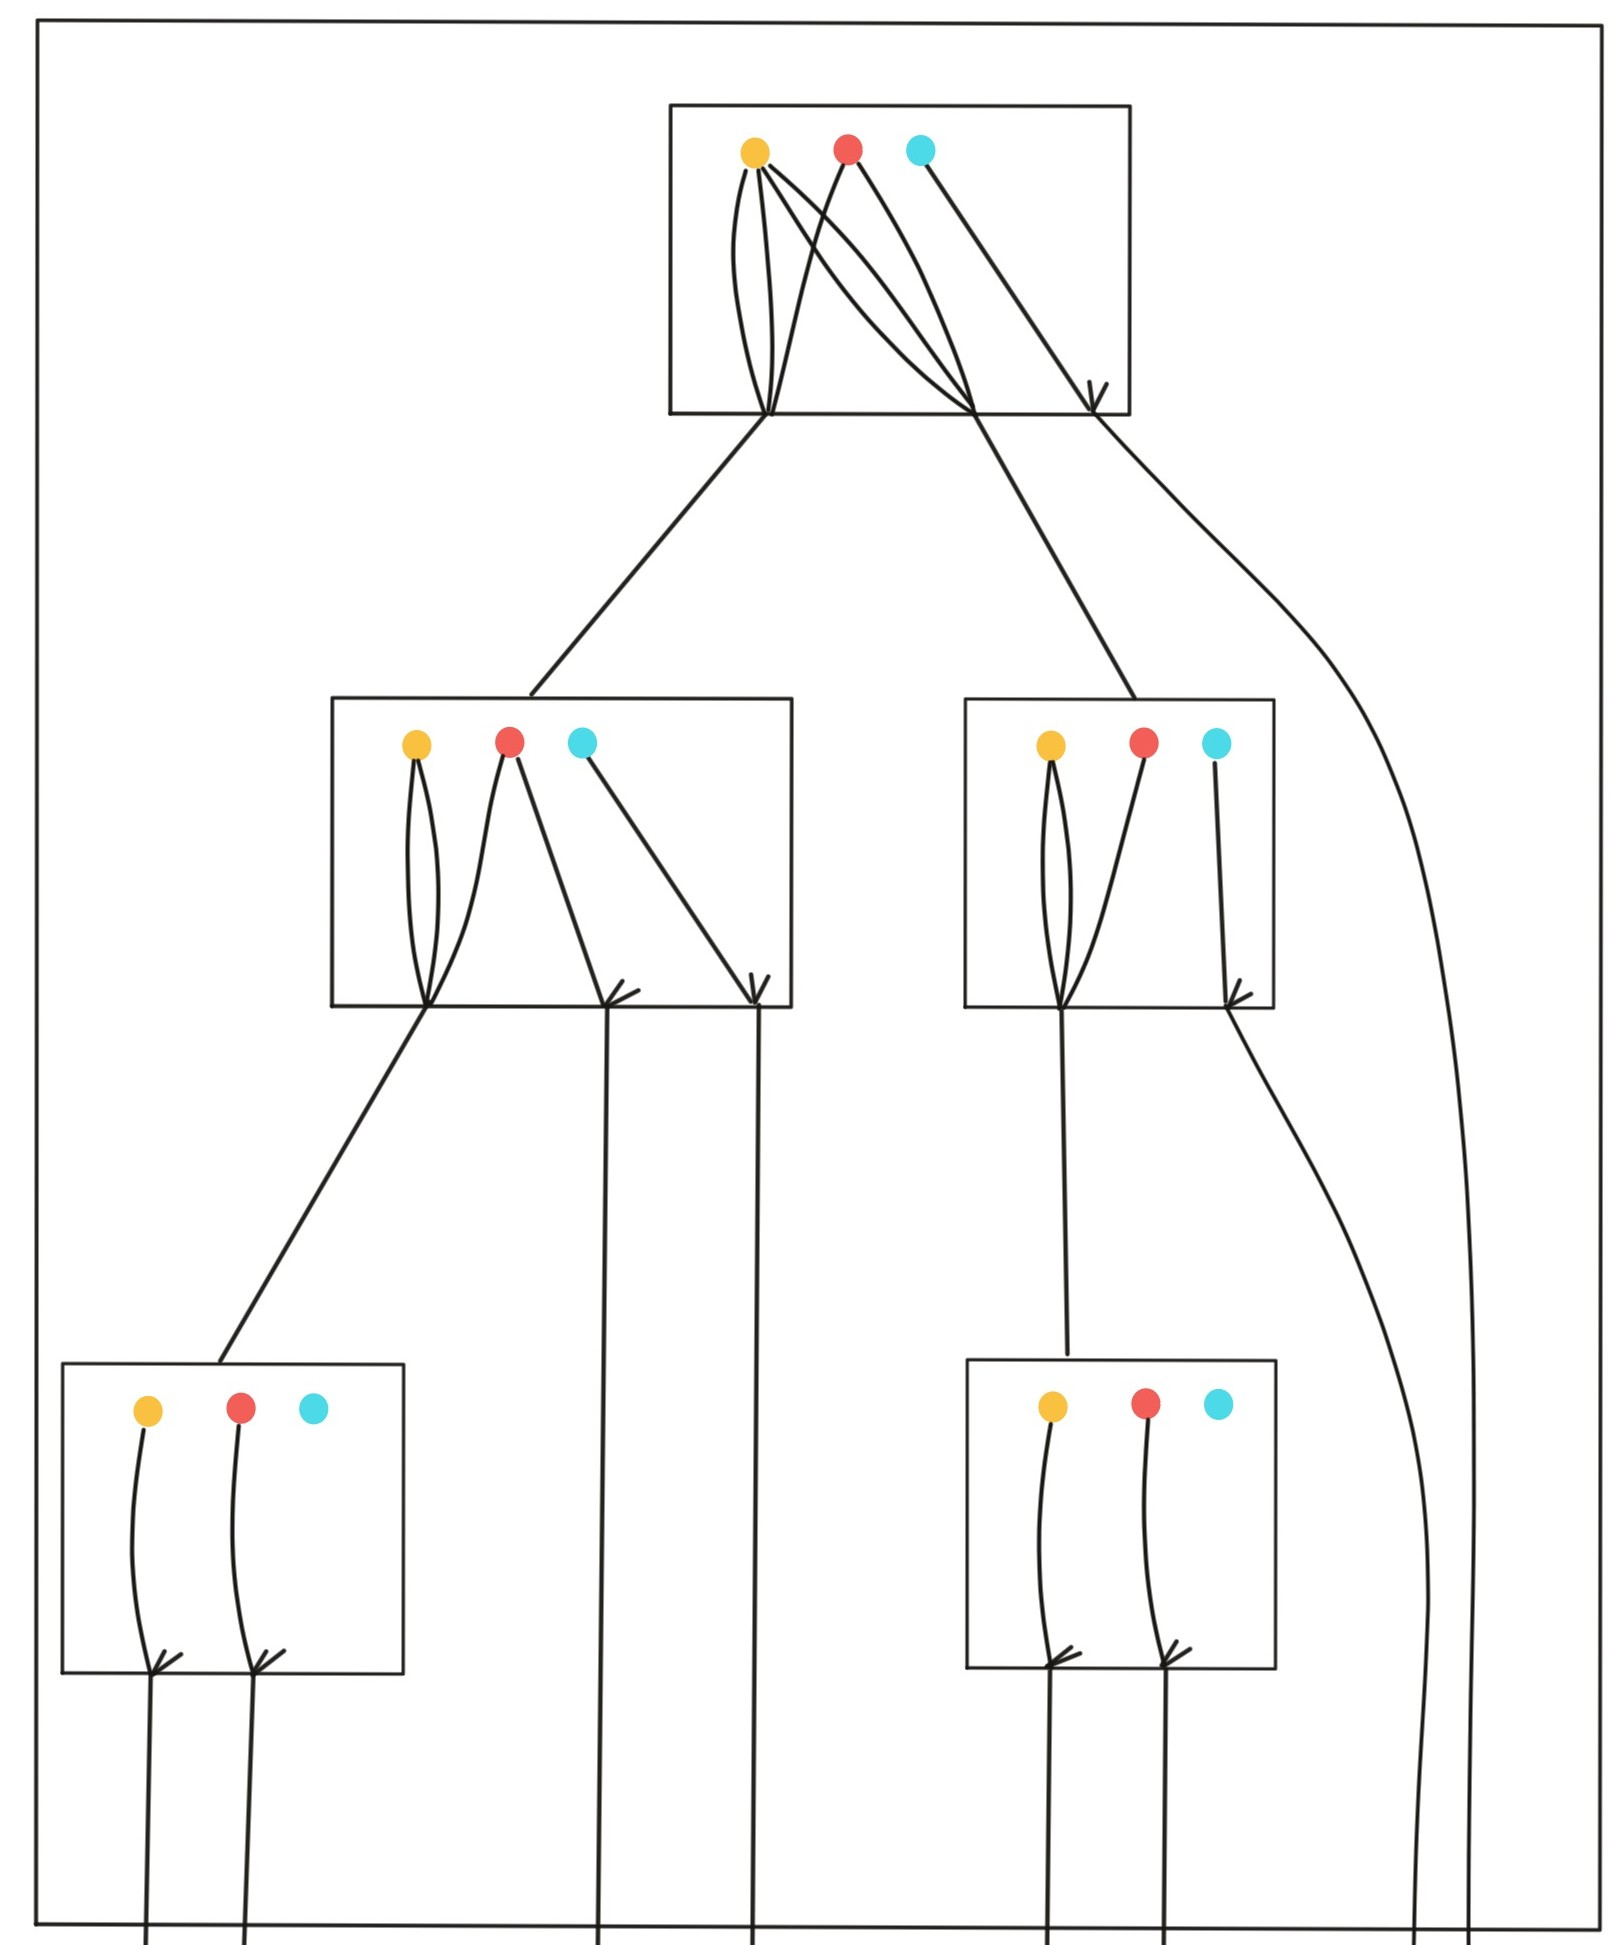
\includegraphics[scale=.1]{MyPic33.jpg}
\end{center} 
Notice that the external twists of our example term have 1 as domain. We can suppose that for all terms under consideration since we can start by applying the function given by lemma~\ref{lem:unfold-external-twist} to unfold the external twists.  Then we proceed in three steps. 
\begin{enumerate}
\item First, we apply the function
\begin{align*}
\ranked{\tmonad \mati k \Sigma \to \reduce k \tmonad(\reduce k\Sigma^{k-1}\otimes \Sigma)}
\end{align*} 
which isolates the last component of the tensor product. We illustrate the effect of the function $f$ by the following example, where $k=3$
\begin{center}
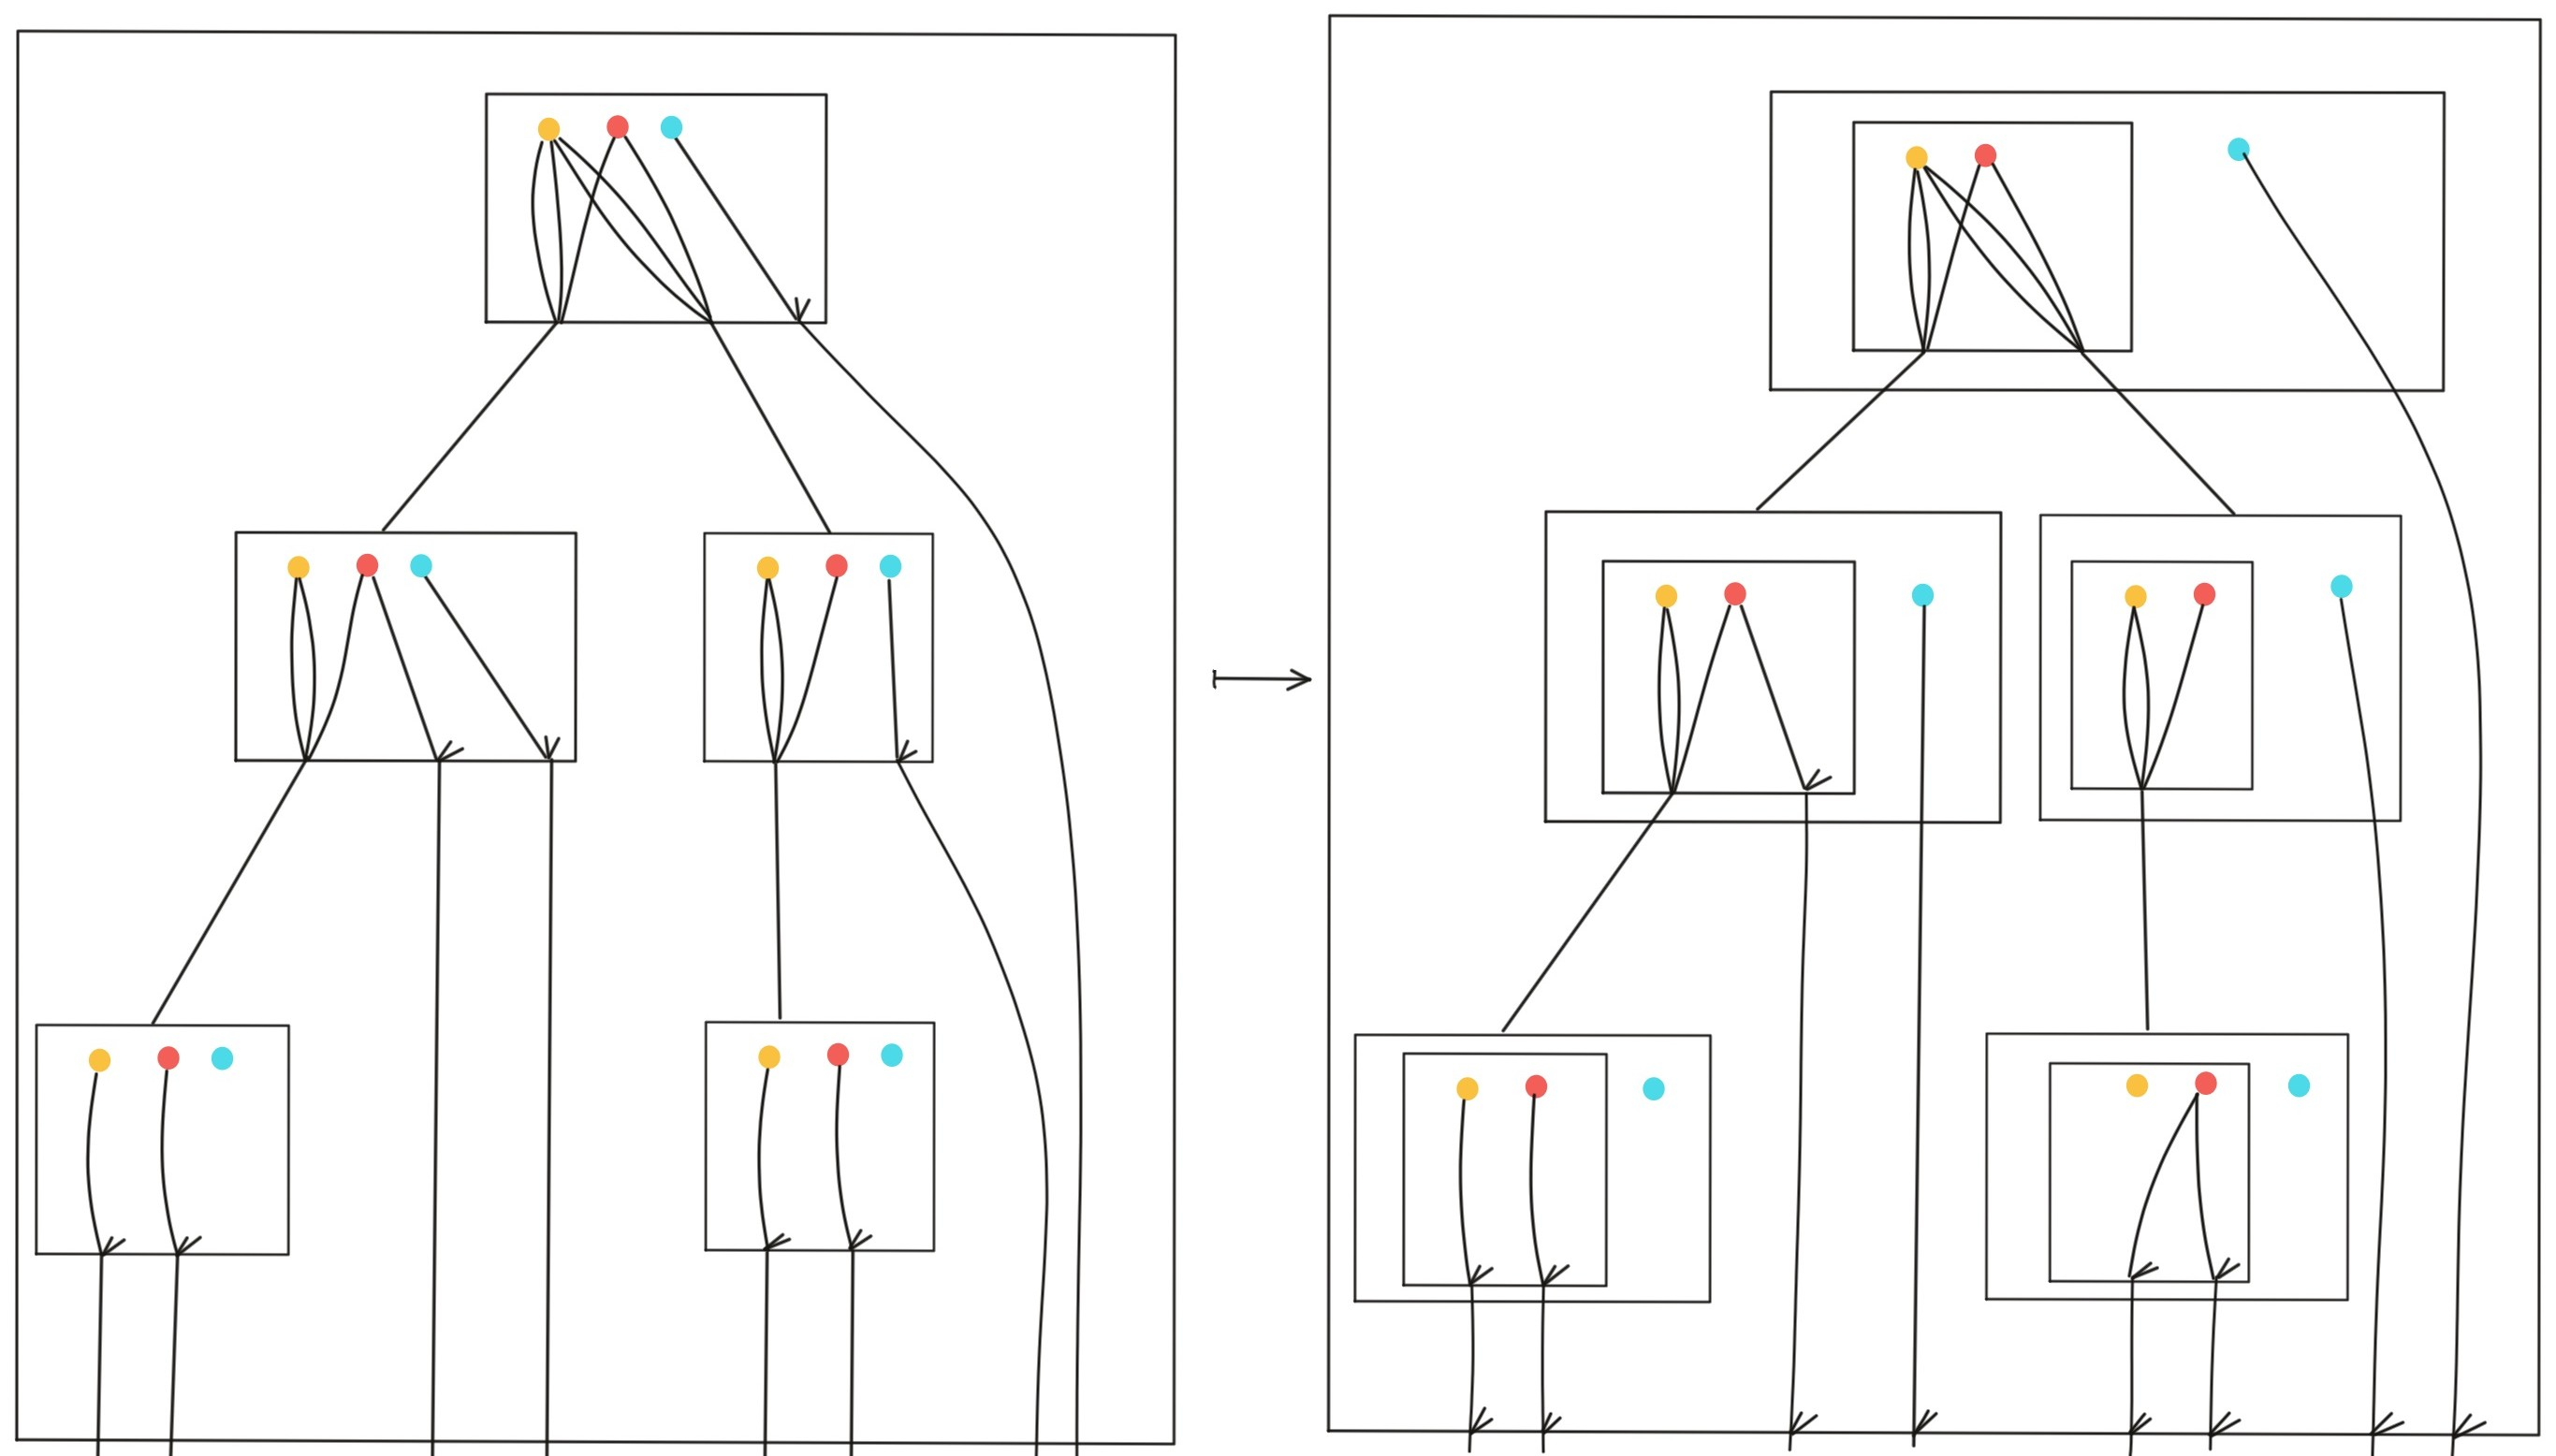
\includegraphics[scale=.1]{MyPic20.jpg}
\end{center}
\item After that, we lift to $\reduce k$ the function function
\begin{align*}
\ranked{\tmonad(\reduce k\Sigma^{k-1}\otimes \Sigma) \to \tmonad\mati {k-1} {(\Sigma\cdot(1+\Sigma))}\otimes \Sigma}
\end{align*}
which pulls-up the last component of the tensor product to the parents, as illustrated by the following picture 
\begin{center}
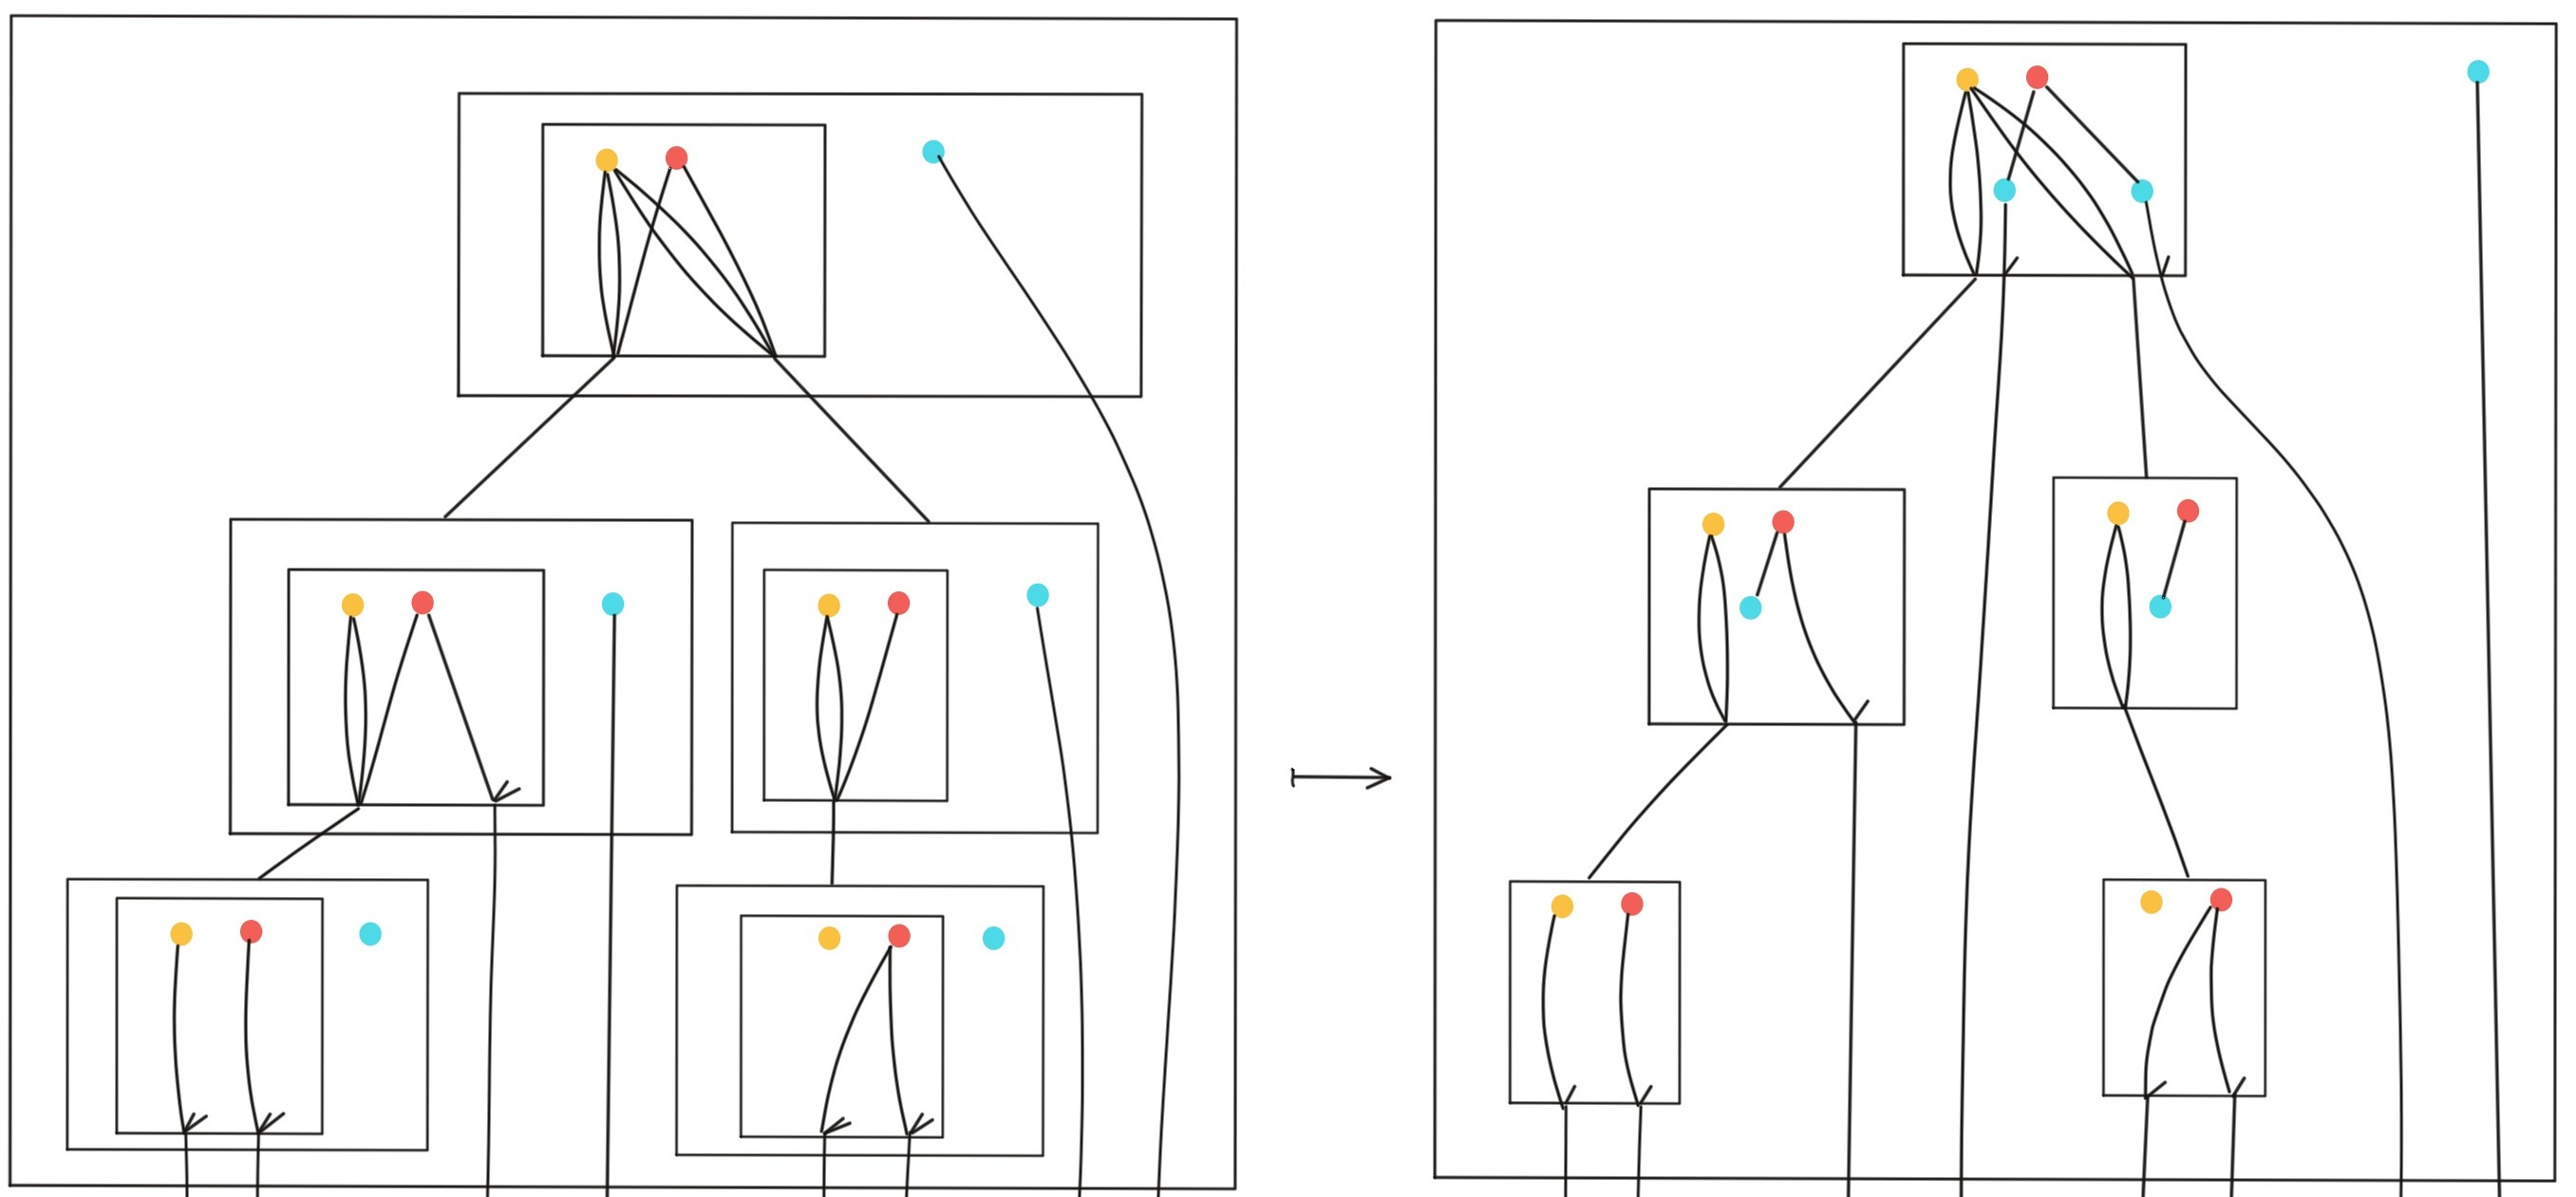
\includegraphics[scale=.12]{MyPic21.jpg}
\end{center}
\item After that, we apply the induction hypothesis to unfold the term from $\ranked{\tmonad\mati {k-1} {(\Sigma\cdot(1+\Sigma))}}$. Finally, after some operations aiming at adjusting the type of the output term, we get our result.
\end{enumerate}
Clearly, the most important steps are 1 and 2. We explain in the following how they can be derived. 

Consider the function 
\begin{align*}
\ranked{f:\tmonad \reduce k (\Gamma\otimes \Sigma)\to \reduce k \tmonad(\reduce k \Gamma\otimes \Sigma)}
\end{align*}
Obtained as follows. First we lift the basic function
\begin{align*}
\ranked { \reduce k (\Gamma\otimes \Sigma) \to  \reduce k (\reduce k \Gamma\otimes \Sigma)}
\end{align*}
to terms. Then we compose the result with the following function, obtained by composing the unfold function with the function of Example~\ref{}
\begin{align*}
 \ranked{\tmonad \reduce k (\reduce k \Gamma\otimes \Sigma) \xrightarrow{\text{Unfold}}
 \reduce k \tmonad (\reduce k \Gamma\otimes \Sigma)\cdot \tmonad \reduce k (\reduce k \Gamma\otimes \Sigma) \xrightarrow{\text{Ex}~\ref{}} \reduce k \tmonad (\reduce k \Gamma\otimes \Sigma)}
\end{align*}
The function of step 1 is the function $\ranked{f}$ where $\ranked{\Gamma}$ is taken to be $\ranked{\Sigma^{k-1}}$.



Now consider the function
\begin{align*}
\ranked{g:\tmonad (\reduce k \Gamma \otimes \Sigma) \to \tmonad \reduce {k-1} (\Gamma\cdot(1+\Sigma))\otimes \Sigma}
\end{align*}
which, for every node (describe). Here is an example illustrating the effect of the function $\ranked{g}$ on the term $t$ below which will be our running example in this proof.
\begin{center}
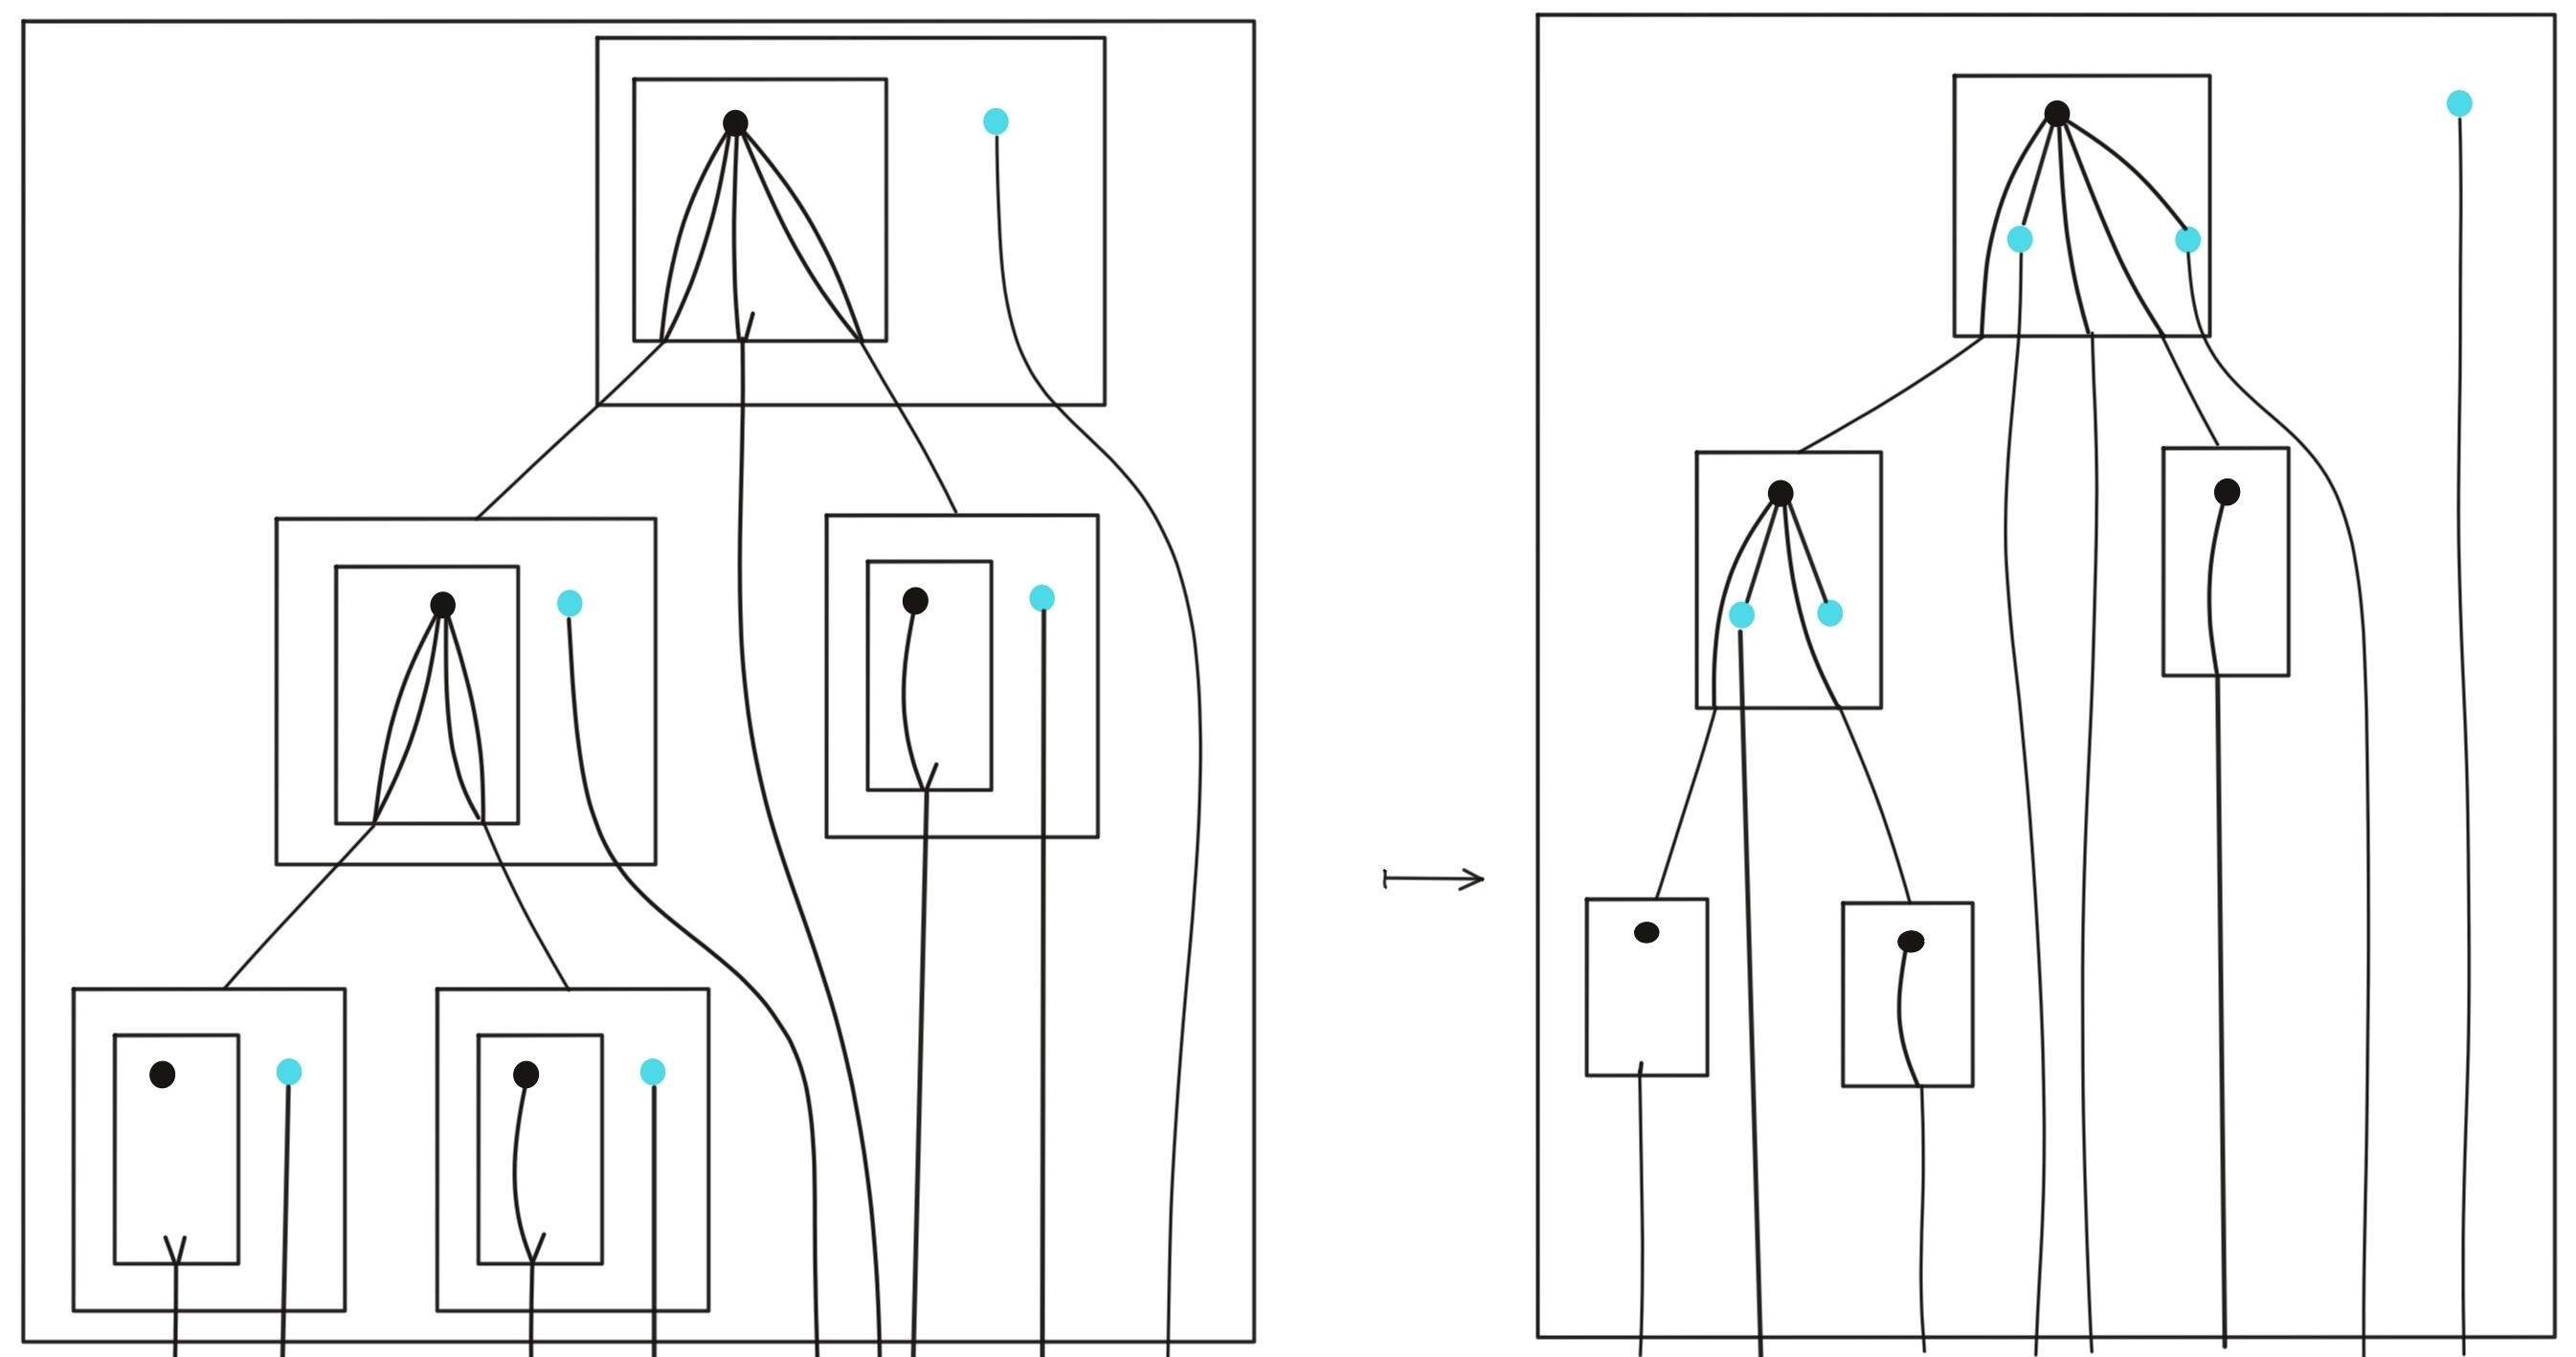
\includegraphics[scale=.12]{MyPic22.jpg}
\end{center}
The function of step 2 is obtained by taking $\ranked{\Gamma}$ to be $\ranked{\Sigma^{k-1}}$ in $\ranked{g}$. Let us see how $\ranked{g}$ can be derived.

First, we embed the tensor product into terms using the derivable function
\begin{align*}
\ranked{\reduce k \Gamma \otimes \Sigma \to \tmonad (2+\reduce k \Gamma +\Sigma)}
\end{align*}
After lifting this function to terms, and flattening the result, we get a term in $\ranked{\tmonad(2+\reduce k \Gamma +\Sigma)}$. 
Consider now the factorisation of these terms
 which is described as follows. There is two types of factors
\begin{itemize}
\item  A factor of the first kind is of depth at most three. Its root is a $\reduce k \rGamma$ element, it contains the children of the root labeled by $2$ and the grand-children labeled by elements from $\rSigma$.
\item If a node is labeled by $2$ or by an element of $\rSigma$, and it is not part of a factor of the first kind, then it forms a singleton factor of its own.    
\end{itemize}
This factorisation is of type
\begin{align*}
\ranked{\tmonad(2+\reduce k \Gamma +\Sigma) \to \tmonad(\reduce k \Gamma\cdot(1+2)\cdot(1+\Sigma)+\tmonad(2+\Sigma+\reduce k \Gamma))}
\end{align*}
Where the type of the first kind of factors is $\ranked{\reduce k \Gamma\cdot(1+2)\cdot(1+\Sigma)}$, the element $1$ is used when a child of the root is not $2$ or a grand child is not an element of $\rSigma$. 
This factrorisation can clearly be implemented by a first-order rational function. After these operations, our example term $t$ becomes like this, where the binary gray node is the element $2$, we omitted the element $1$ in the figure, and the factorisation is indicated by the red lines
\begin{center}
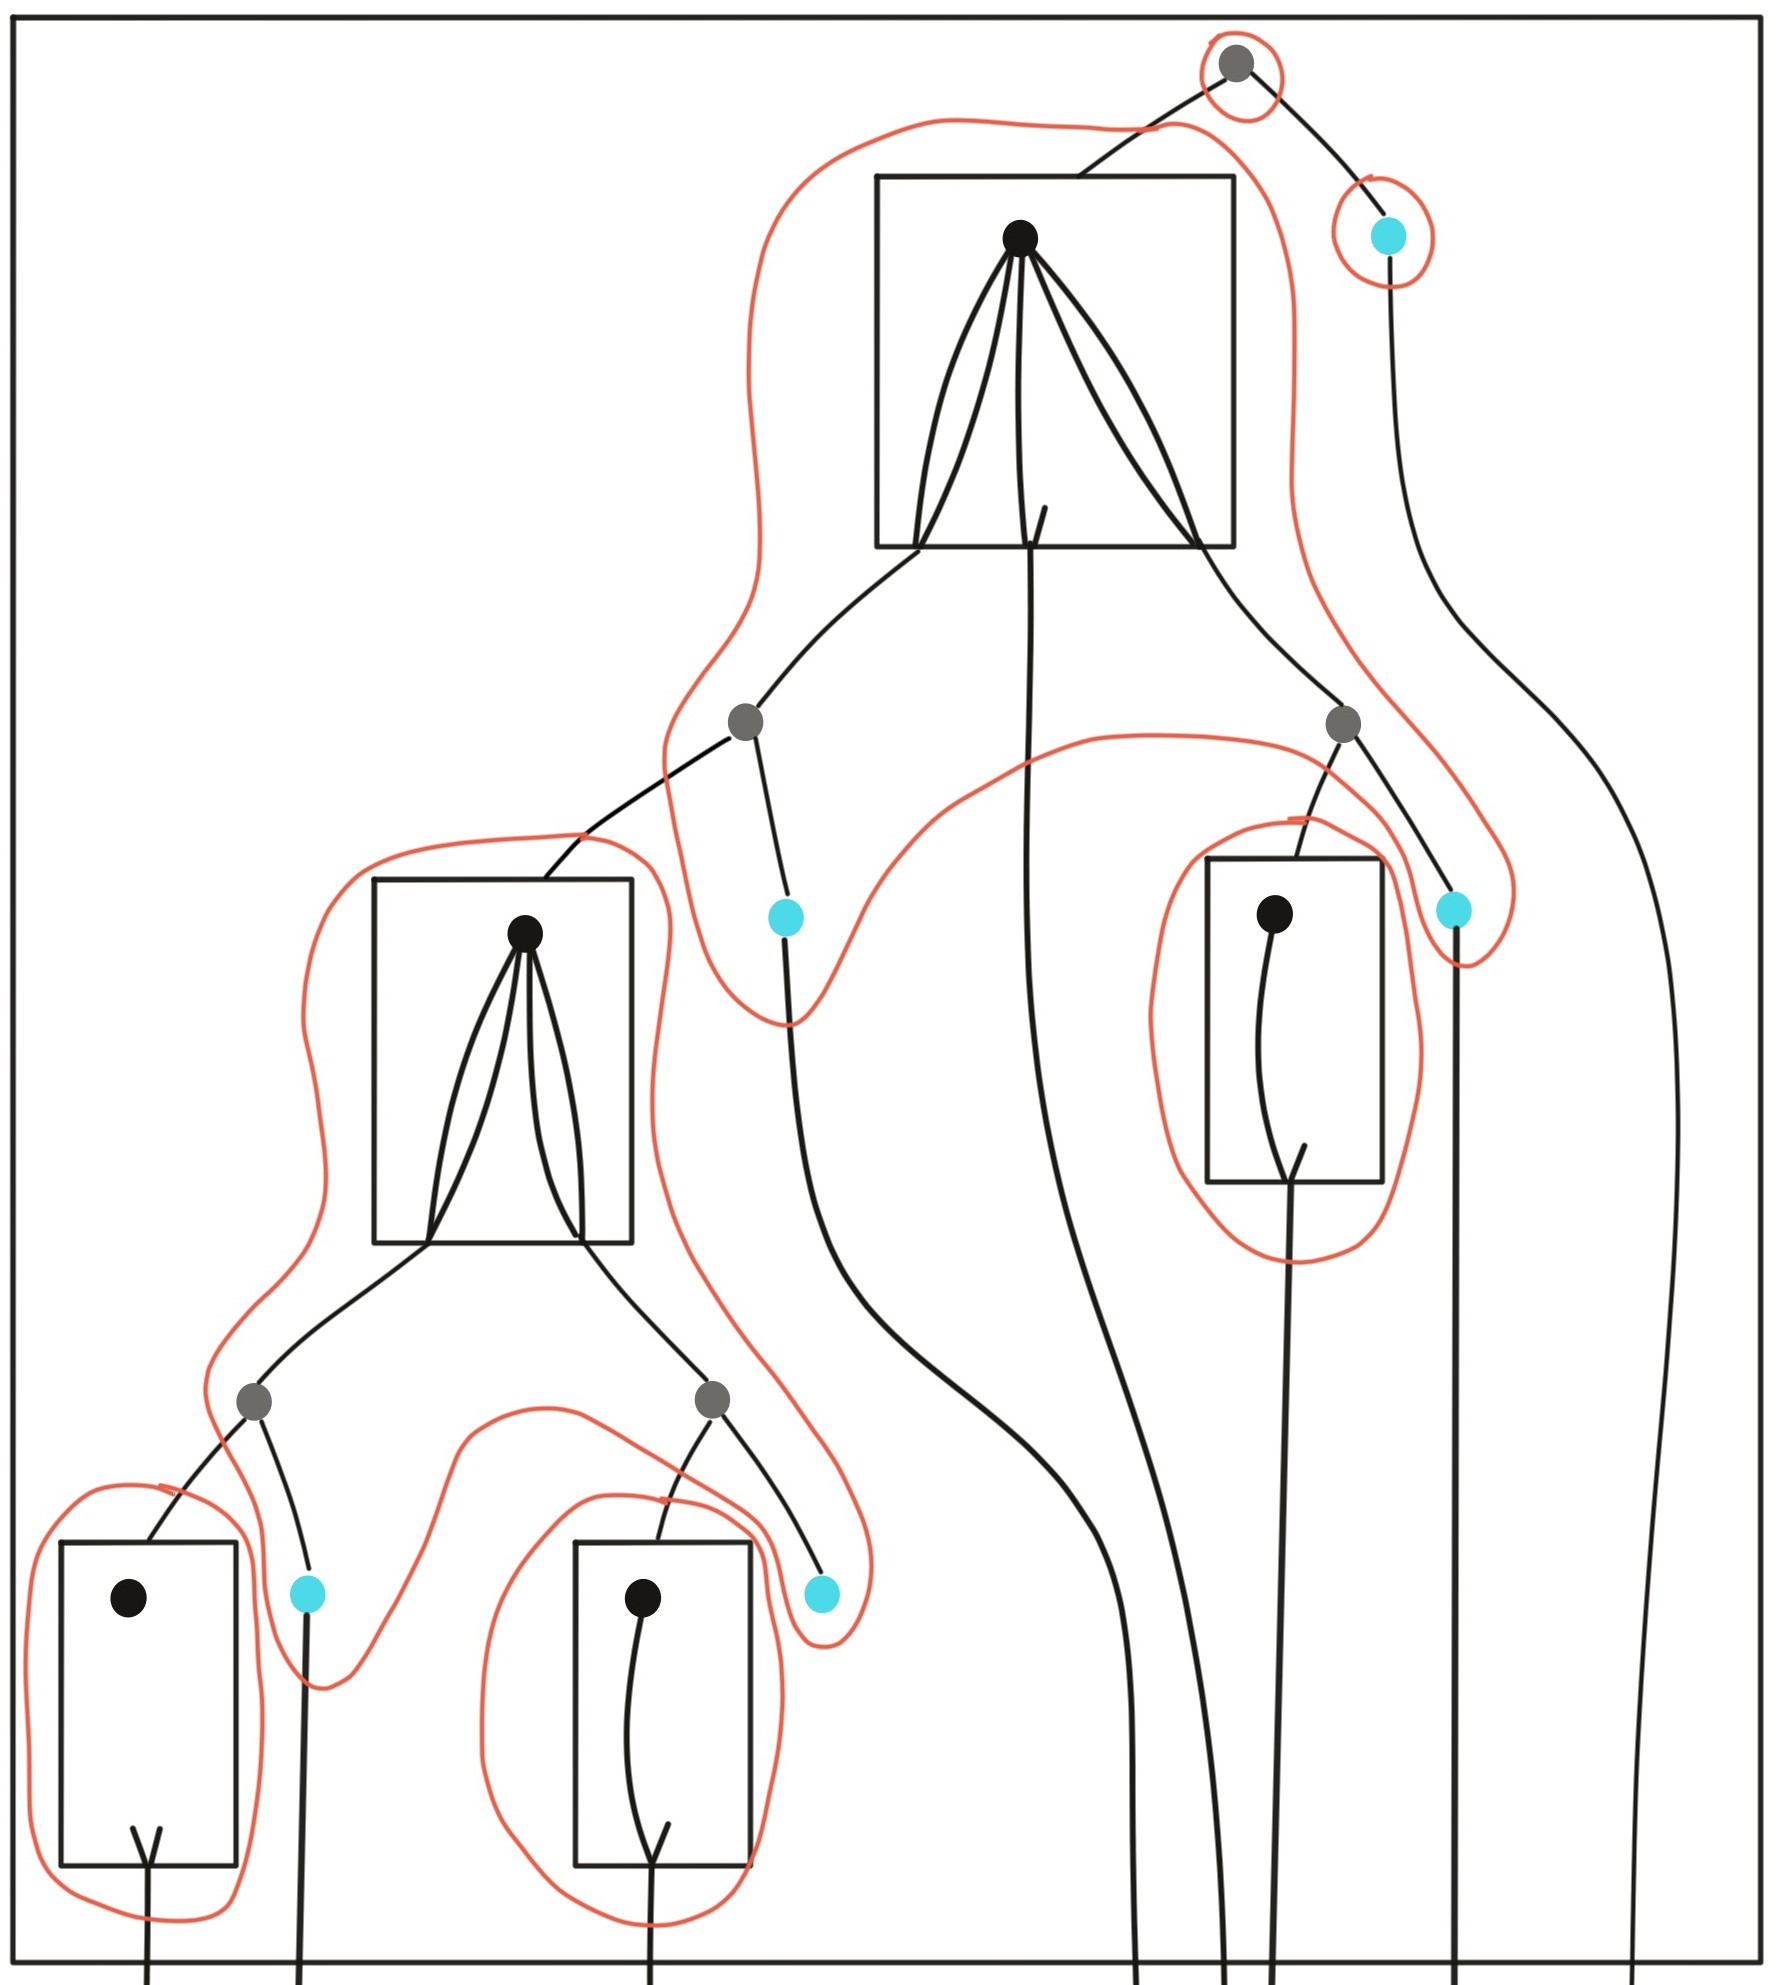
\includegraphics[scale=.09]{MyPic23.jpg}
\end{center}
  After that, we apply to each block of the first kind the homomorphism that transforms every element $2$ into the following element of type $\ranked{\mati k 1}$
  \begin{center}
  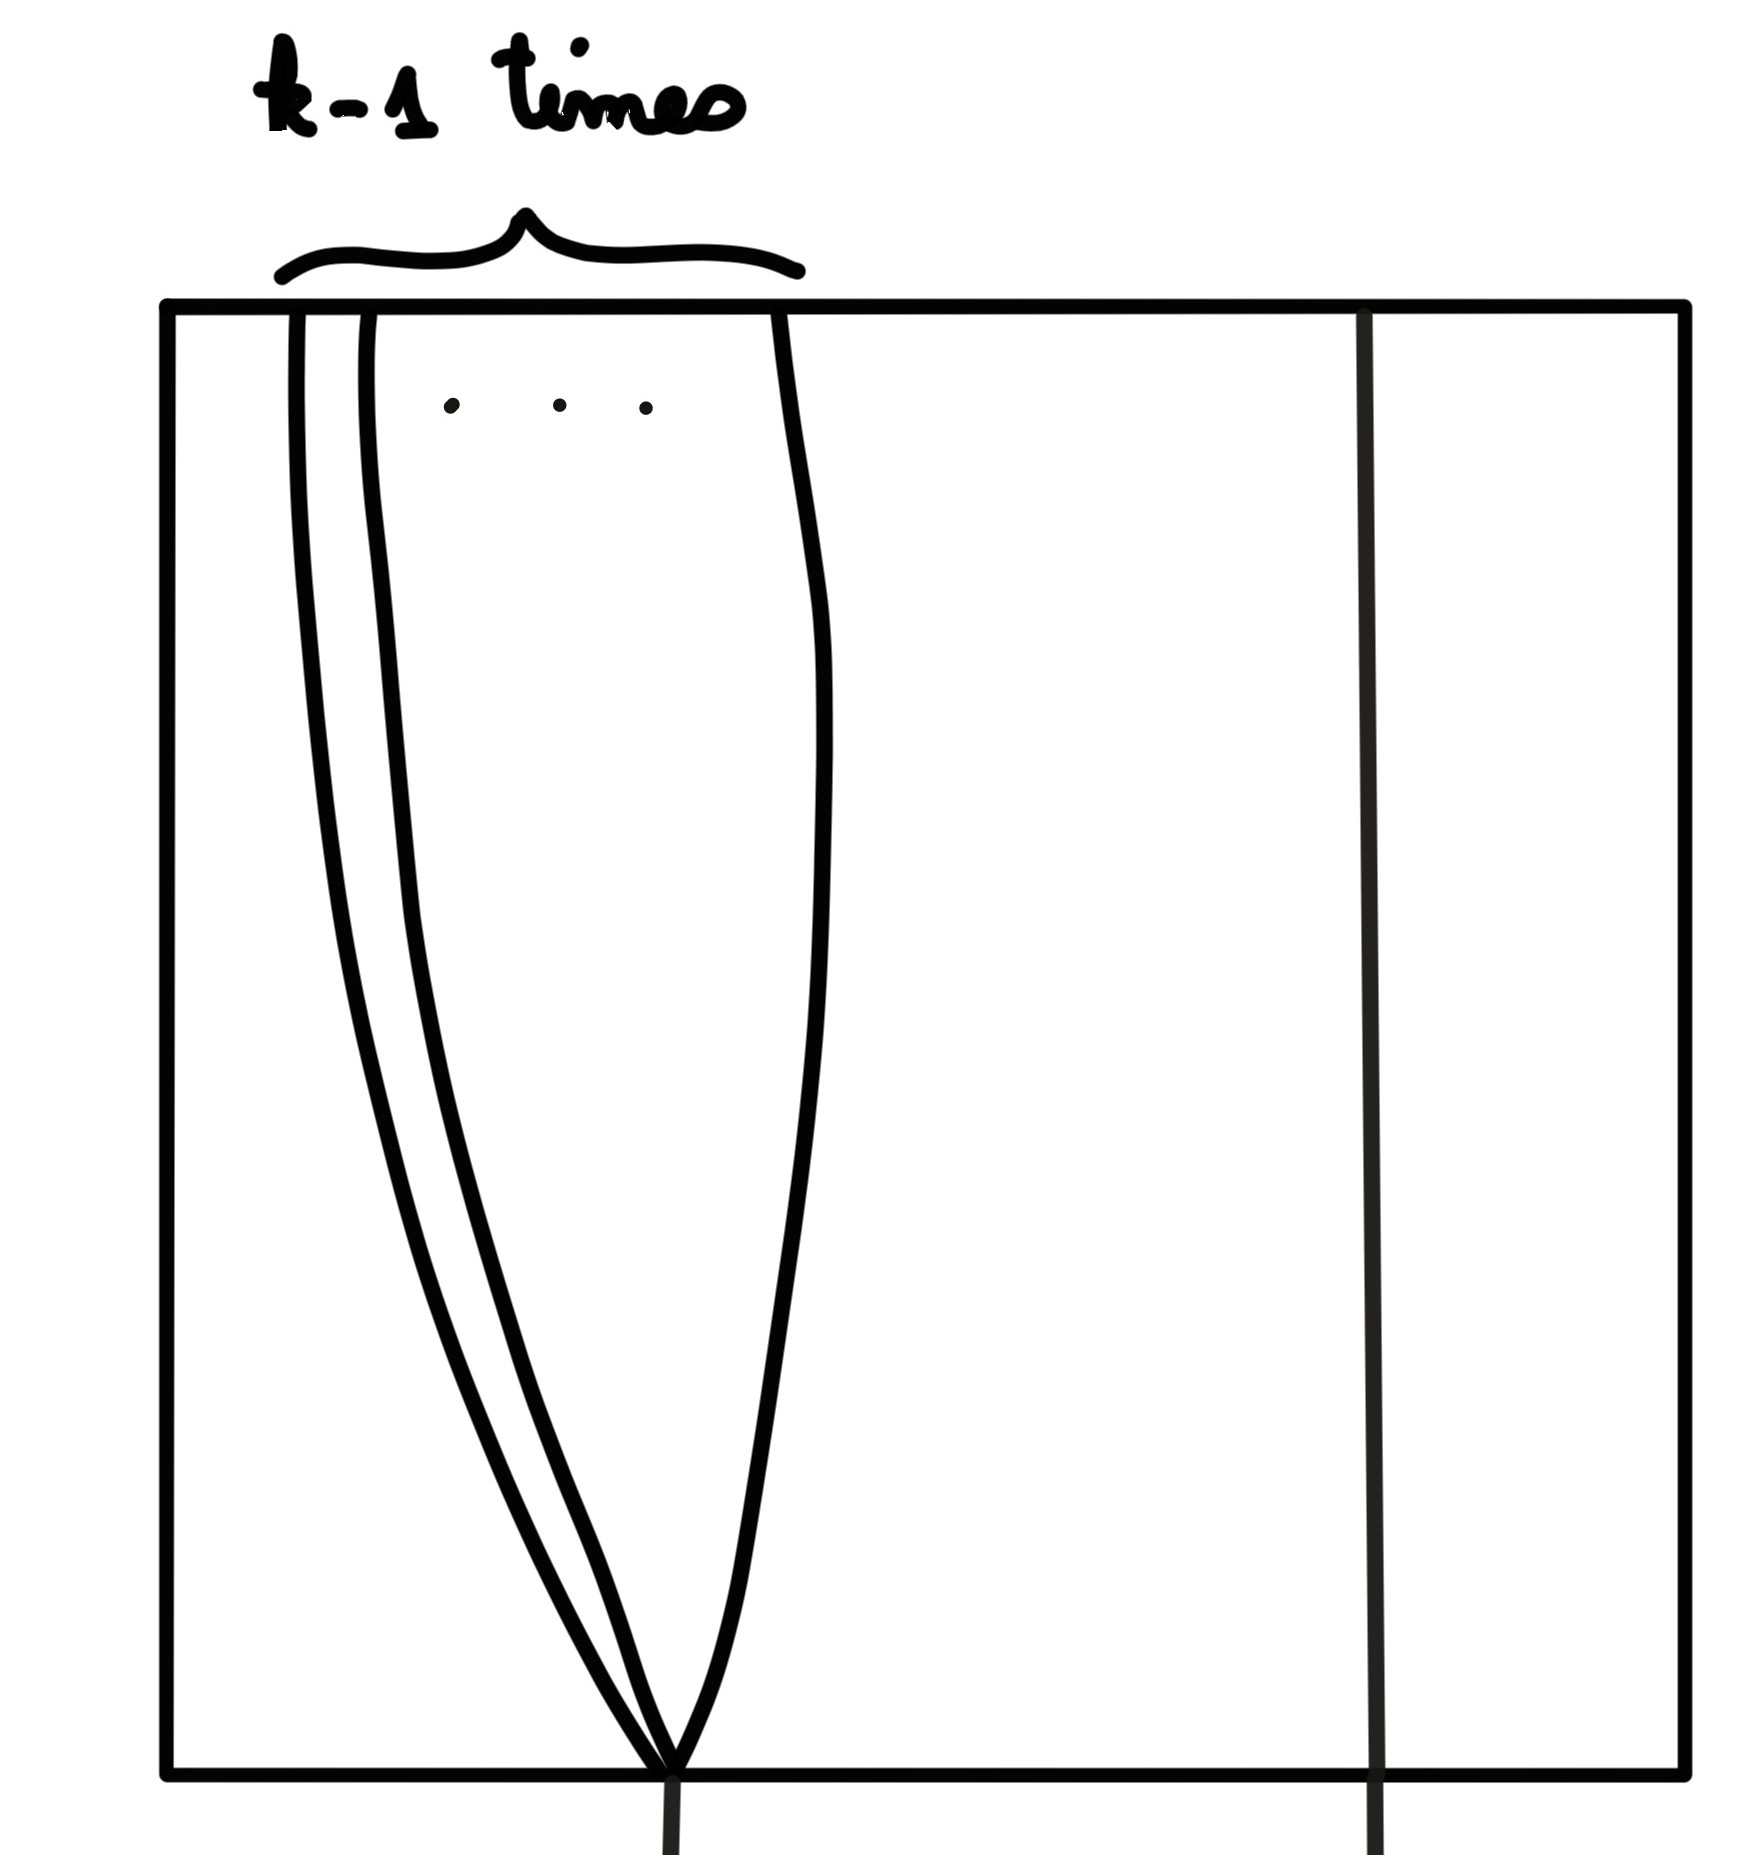
\includegraphics[scale=.03]{MyPic24.jpg}
  \end{center}
  and keeps the other nodes unchanged. The term $t$ becomes now
  \begin{center}
  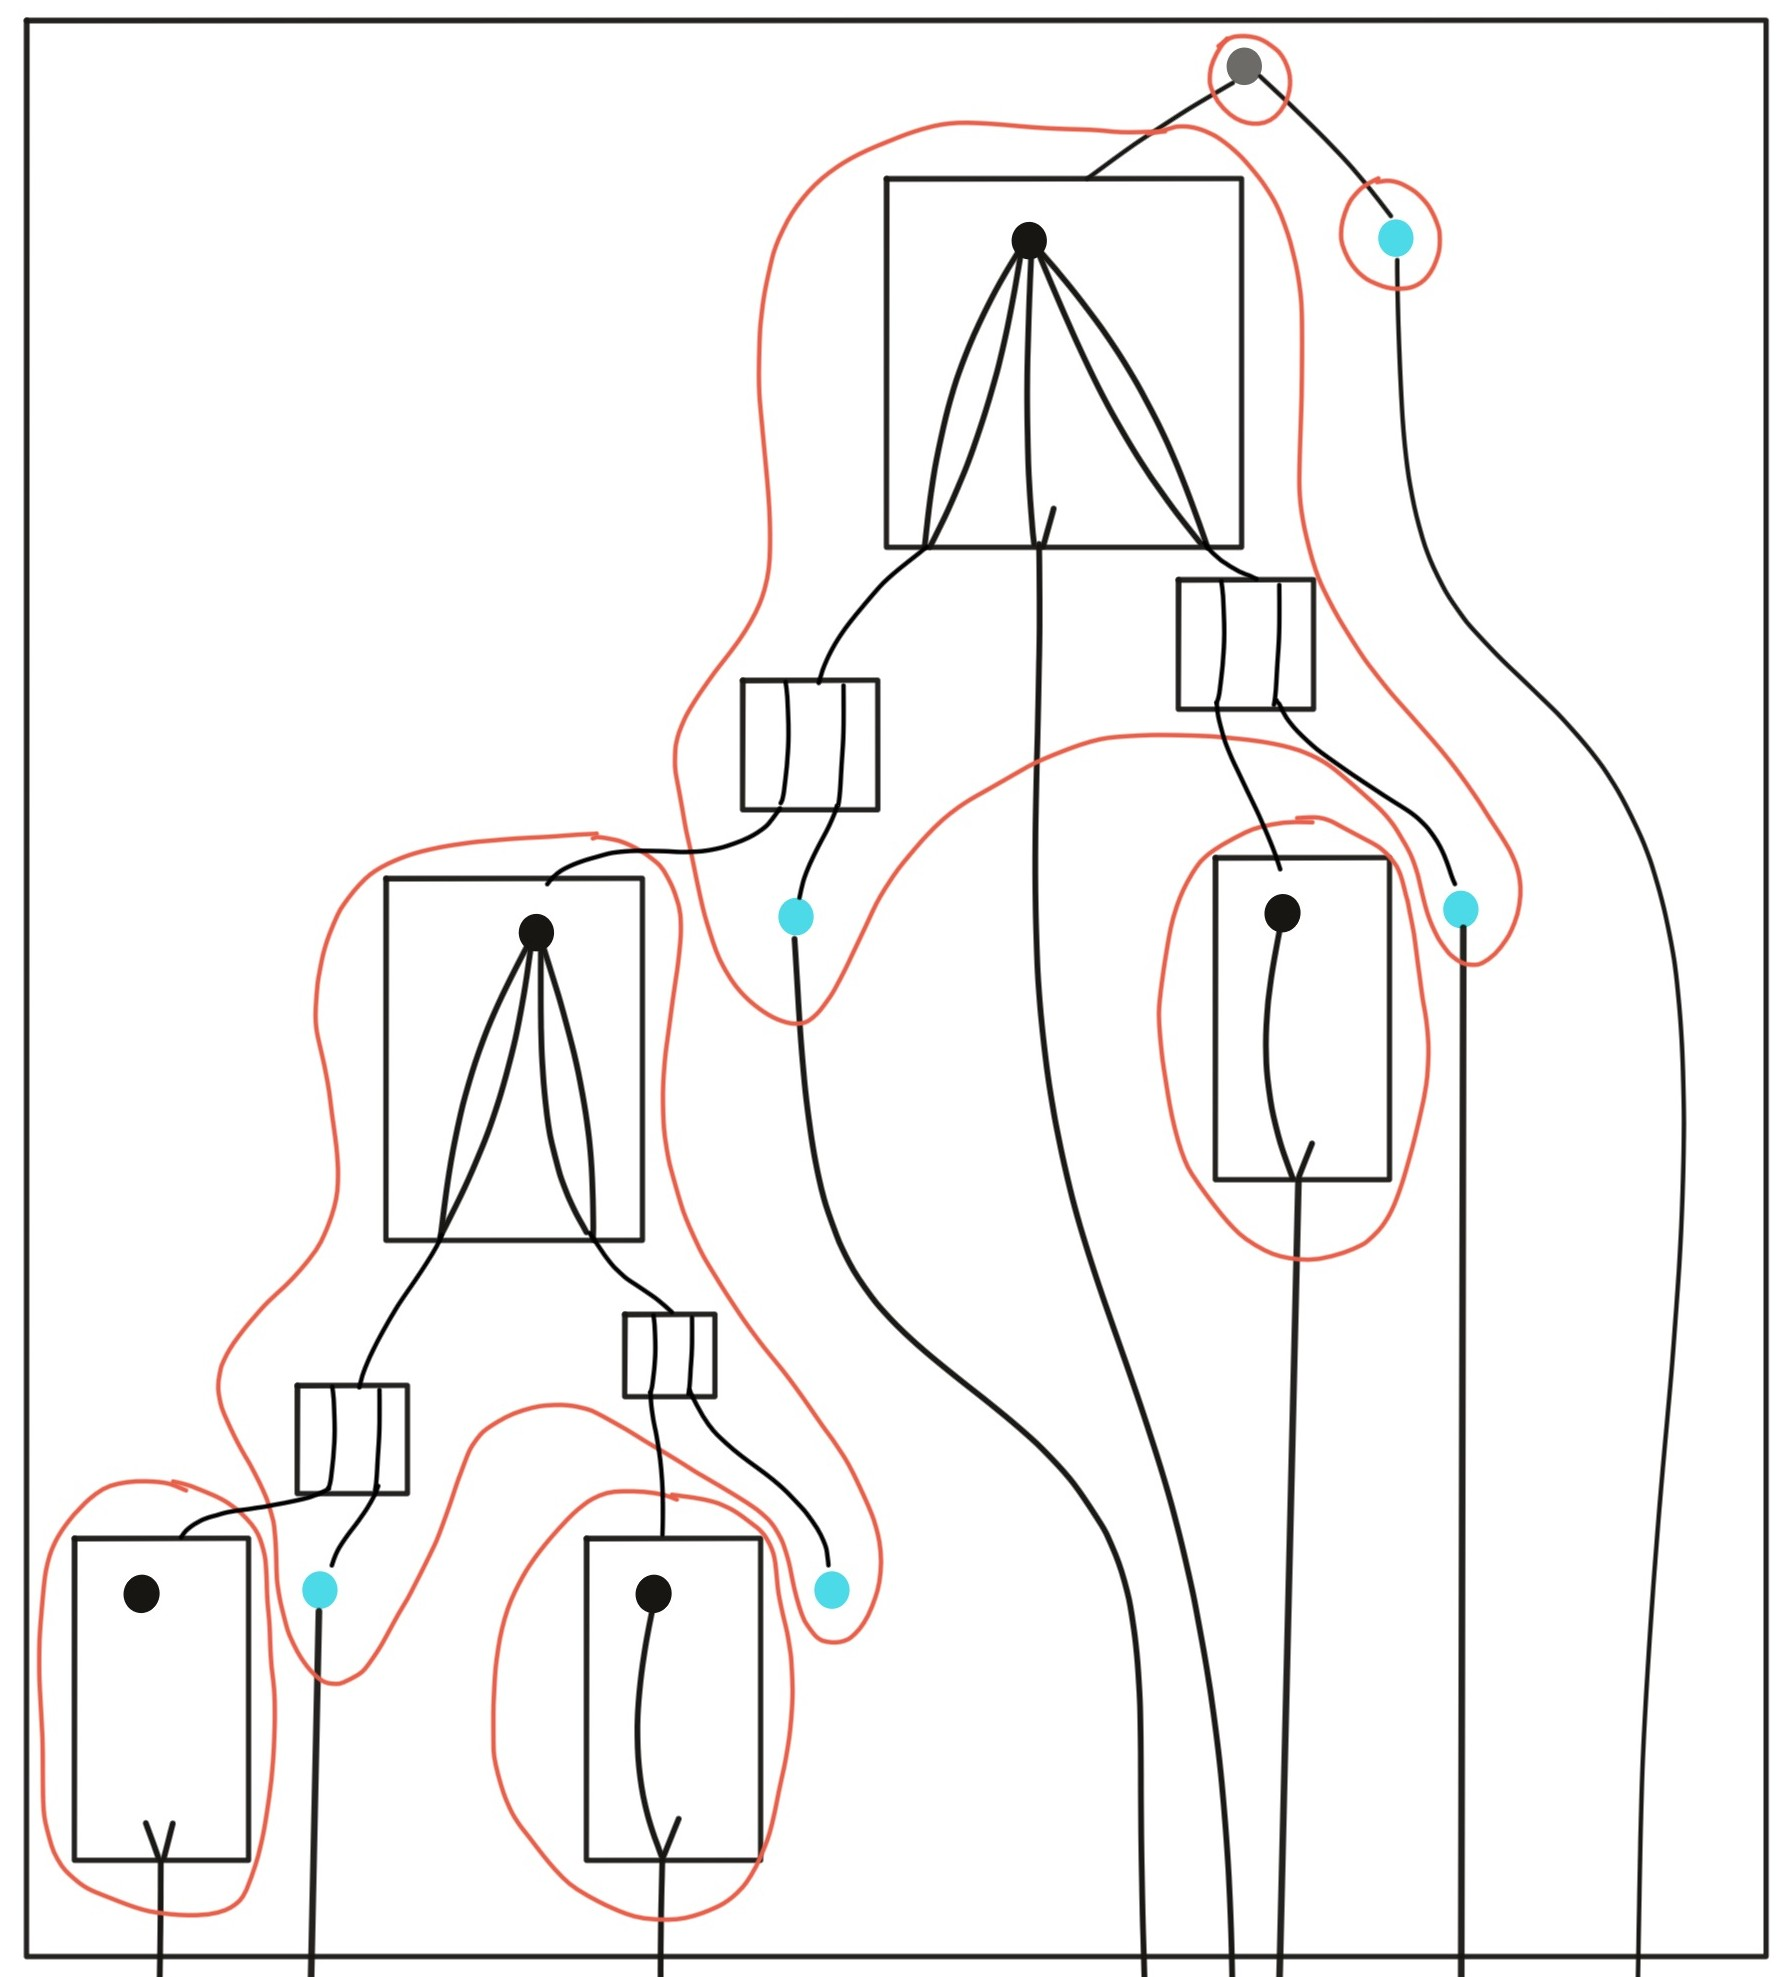
\includegraphics[scale=.09]{MyPic25.jpg}
  \end{center}
  We can now lift the partial shallow unfold (Example~\ref{}), followed by an injection and the elimination of $1$ to recover the type $\ranked{\reduce k \Gamma}$
  \begin{align*}
  \ranked{\reduce k \Gamma\cdot(1+\mati k 1)\to \reduce k (\Gamma\cdot(1+1))\to \reduce k (\Gamma\cdot 1) \to  \reduce k \Gamma}
\end{align*}
which result into a term of type $\ranked{\tmonad(\reduce k\Gamma\cdot(1+\Sigma)+\tmonad(2+\Sigma+\reduce k \Gamma))}$. We apply then the following basic functions, which aims at putting the $\cdot$ inside the scope of $\reduce k$, then reducing the degree of the fold:
\begin{align*}
\ranked{\reduce k\Gamma\cdot(1+\Sigma)\to \reduce k(\Gamma\cdot(1+\Sigma))\to \reduce {k-1}(\Gamma\cdot(1+\Sigma)\cdot (0+1)) }
\end{align*}
After that, we apply some flattening to get the desired term. However, we still do not have the right type. I need either a bottom, or something else to handle the garbage.
\end{proof}


\subsubsection{Term unfolding for homogeneous inputs}
\label{subsec:something-homo-unfold}
we say that a term $ t \in \tmonad \mati k \rSigma$ is homogeneous if for every two internal branches $b_1, b_2$ having twists $\alpha_1, \alpha_2$ respectively and such that $b_2$ is a child of $b_1$, we have that
\begin{align*}
\alpha_1\alpha_2=\alpha_1
\end{align*}

The rest of this section is devoted to proving the following lemma. 

\begin{lemma}\label{lem:homo-2-twist}
    Let $k \in \set{1,2,\ldots}$. There is a derivable operation 
    \begin{align*}
        \ranked{f : \tmonad \mati k \rSigma \to \mati k {(\tmonad \Sigma)} }
        \end{align*}      
which coincides with term unfolding for all inputs which are homogeneous.
\end{lemma}
To perform the unfolding of homogeneous inputs, we need the following function
\begin{align*}
\ranked{\reduce k \Sigma^l \to \reduce 1 (\reduce k \Sigma\cdot(0+1))^l }
\end{align*}
which plugs $0$ to the folds shared by two distinct elements of the tensor product
\begin{center}
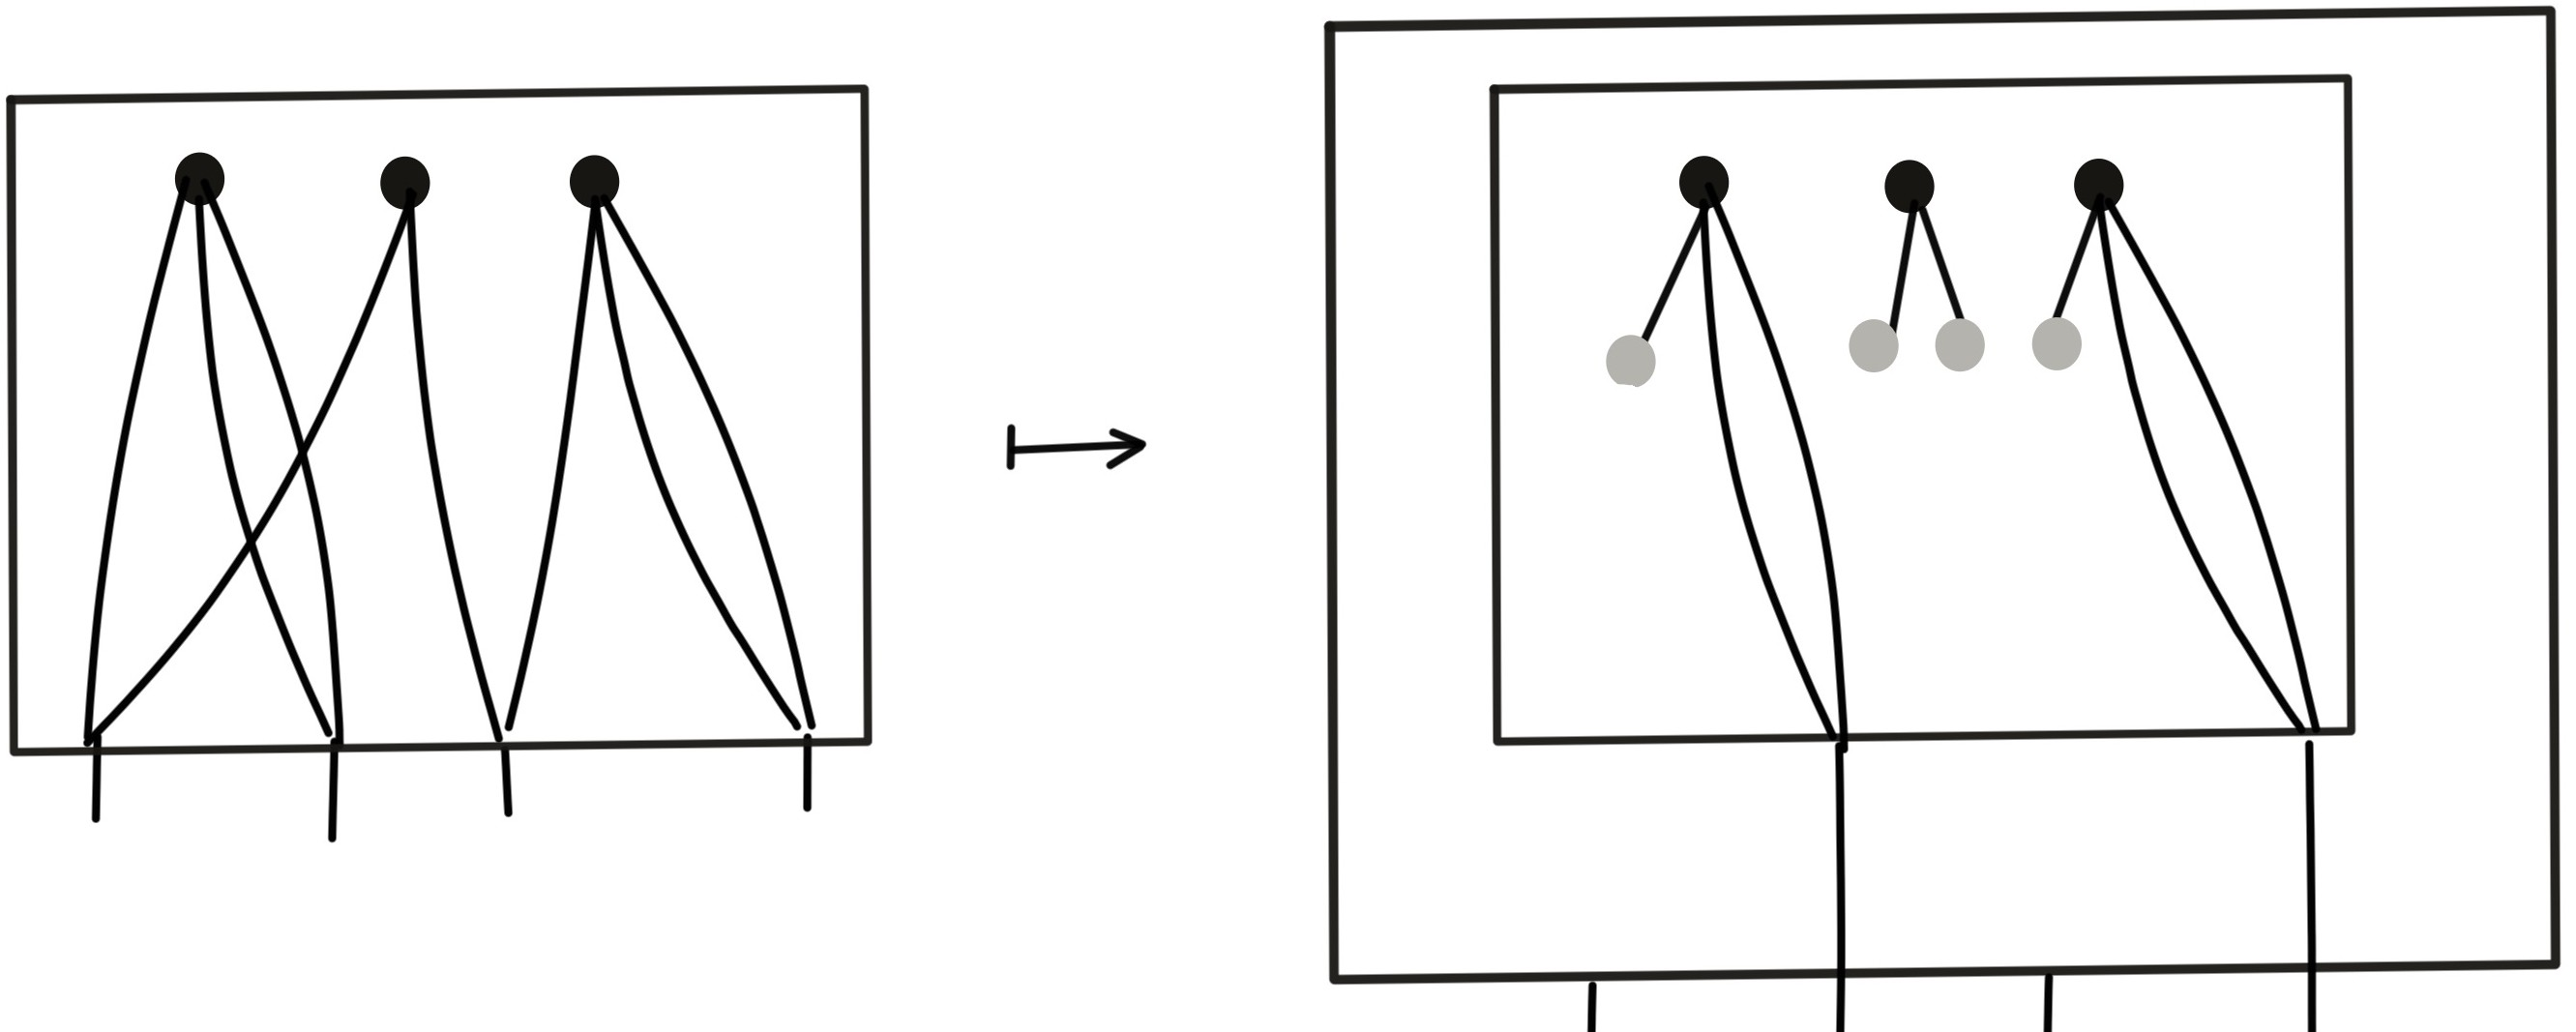
\includegraphics[scale=.07]{MyPic34.jpg}
\end{center}

\begin{lemma}
Let
\begin{align*}
\alpha:\set{1,\dots,k}\to\set{1,\dots,k}\qquad
\beta:\set{1,\dots,k}\to\set{1,\dots,k}
\end{align*} 
be two monotone functions such that
\begin{align*}
\alpha\beta=\alpha
\end{align*}
\begin{itemize}
\item If the graph of $\alpha$ is not weakly connected, then so is the graph of $\beta$. 
\item Moreover, if $m\in \set{1,\dots, k}$ is such that 
\begin{align*}
\alpha\set{1,\dots,m}\subseteq \set{1,\dots,m} \qquad \text{and}\qquad 
\alpha\set{m+1,\dots,k}\subseteq \set{m+1,\dots,k}
\end{align*}
then we have also 
\begin{align*}
\beta\set{1,\dots,m}\subseteq \set{1,\dots,m} \qquad \text{and}\qquad 
\beta\set{m+1,\dots,k}\subseteq \set{m+1,\dots,k}
\end{align*}
\item If the graphs of $\alpha$ and $\beta$ are both weakly connected, then the image of $\alpha$ and the image of $\beta$ are both singletons.
\end{itemize}
\end{lemma}

\begin{proof}[Proof of Lemma~\ref{lem:homo-2-twist}]
~\\
\begin{center}
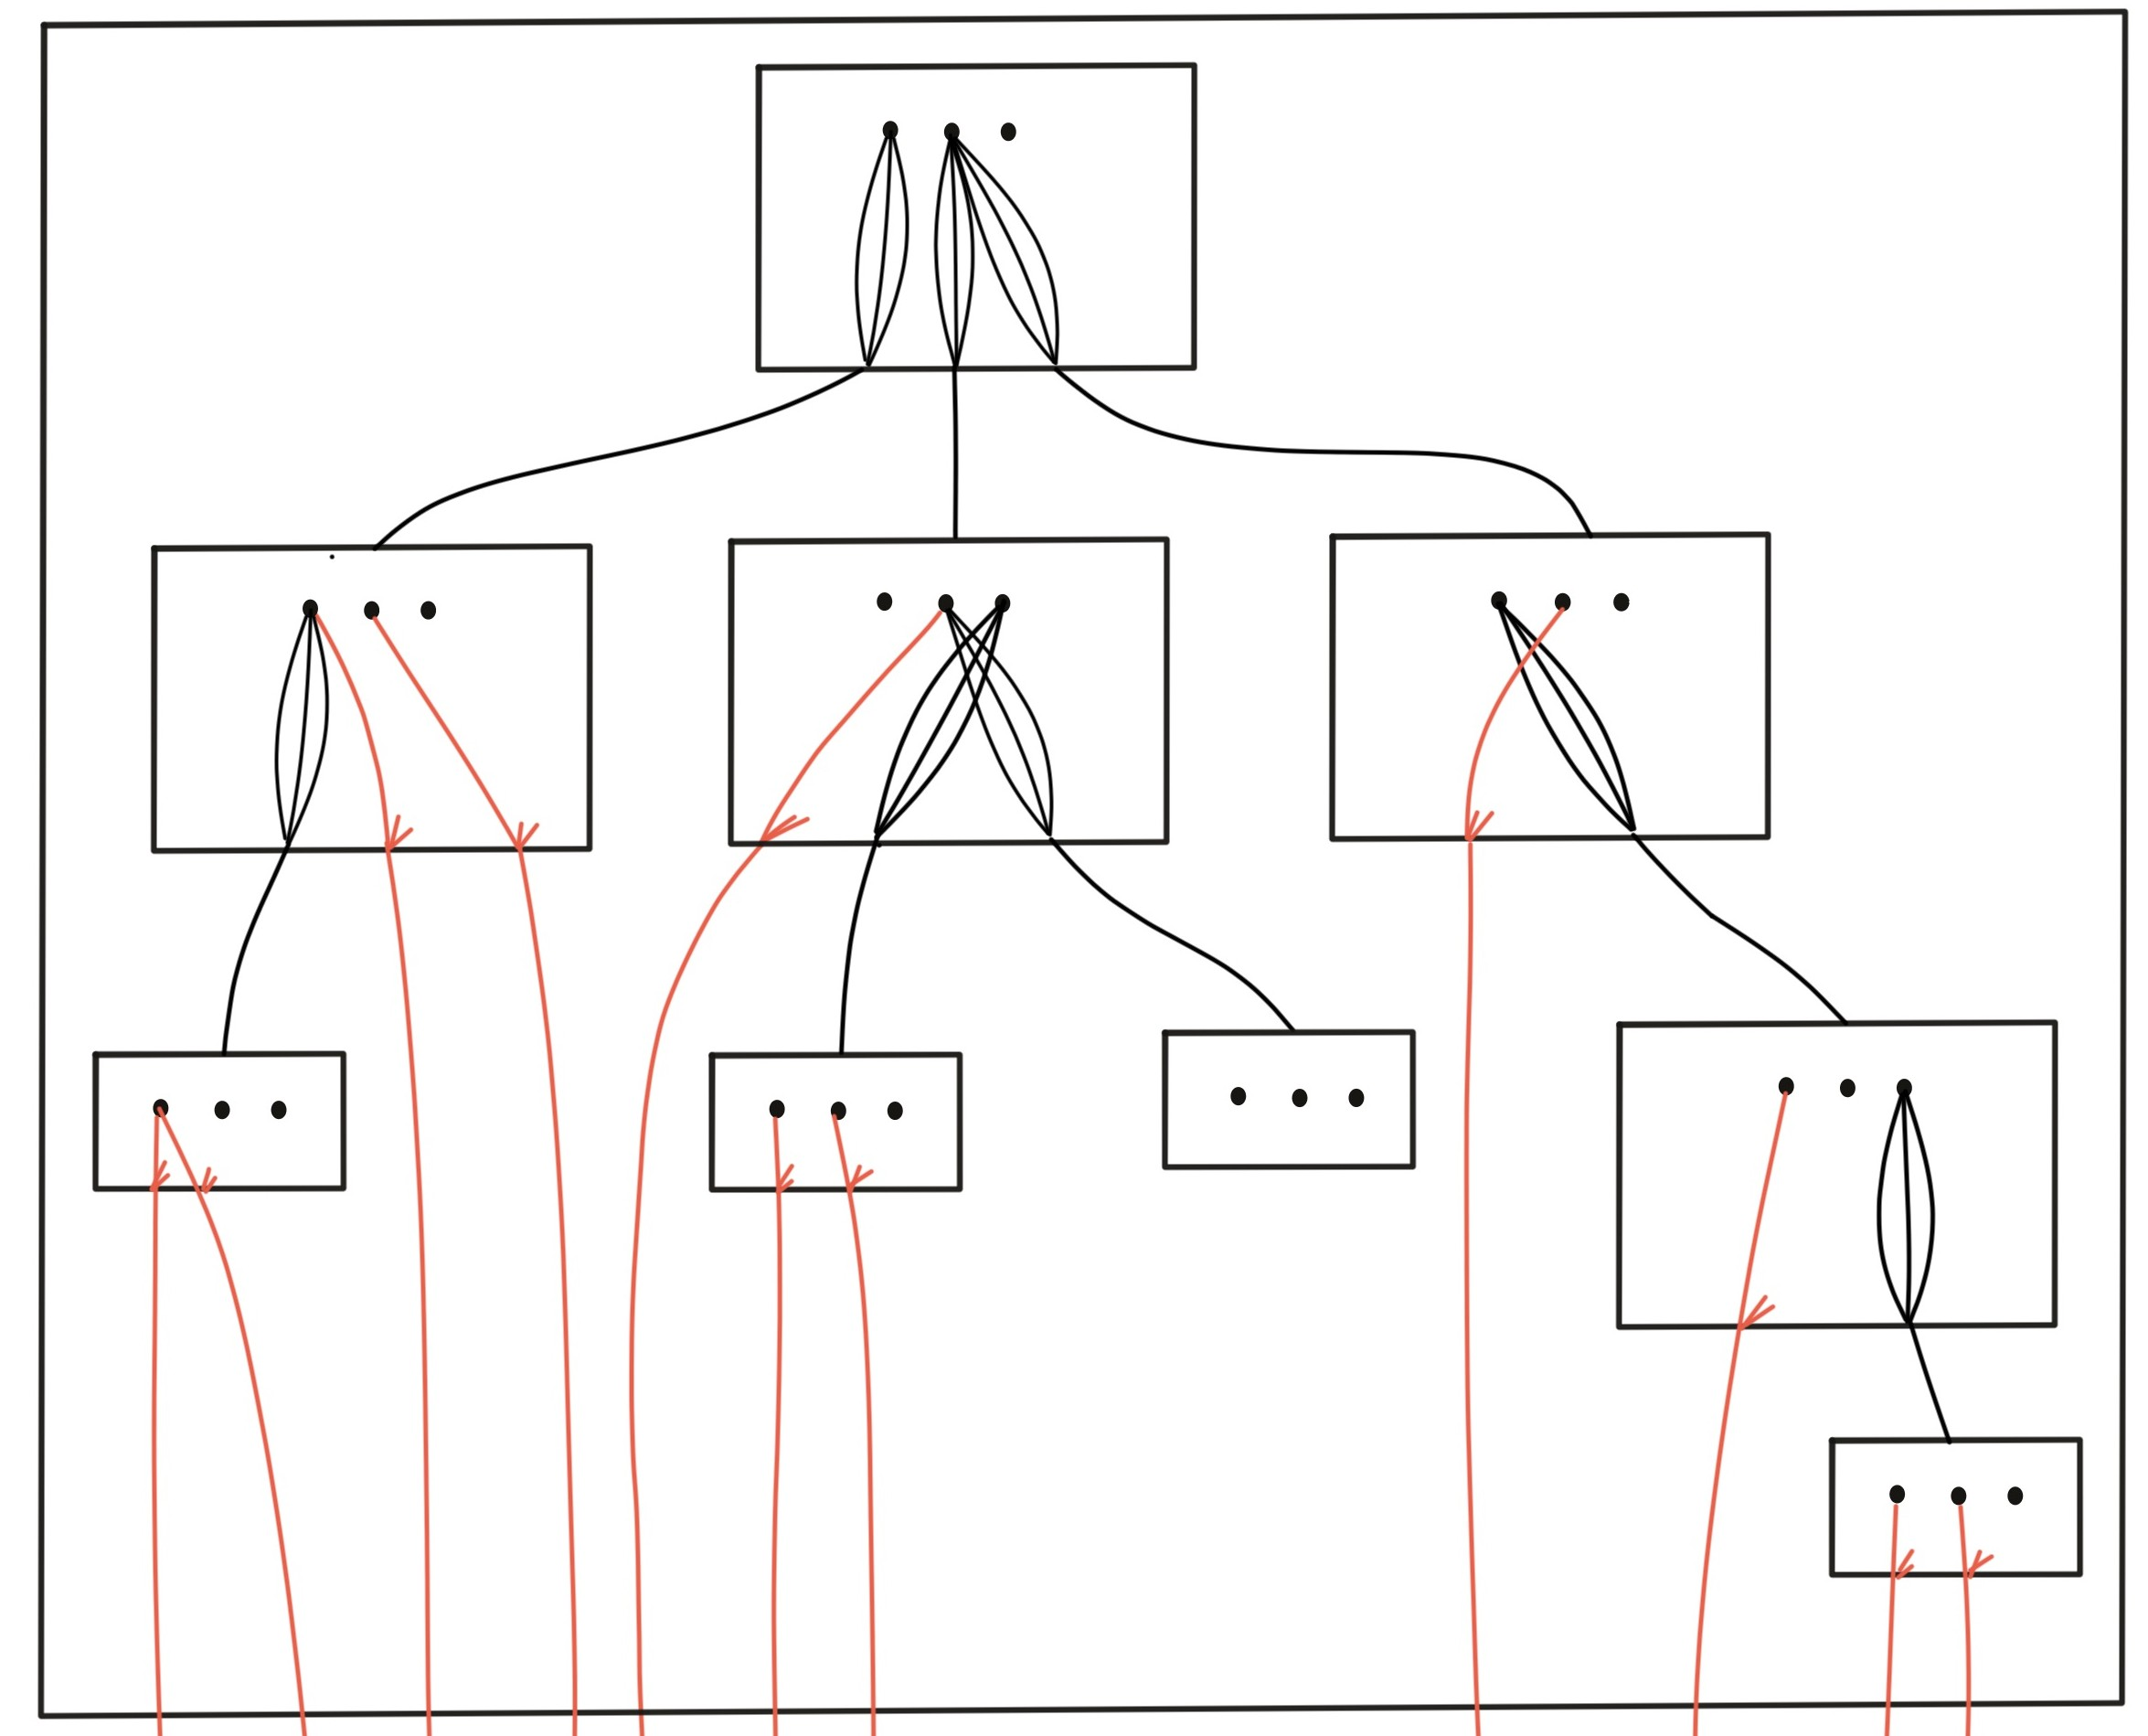
\includegraphics[scale=.07]{MyPic35.jpg}
\end{center} 
\begin{center}
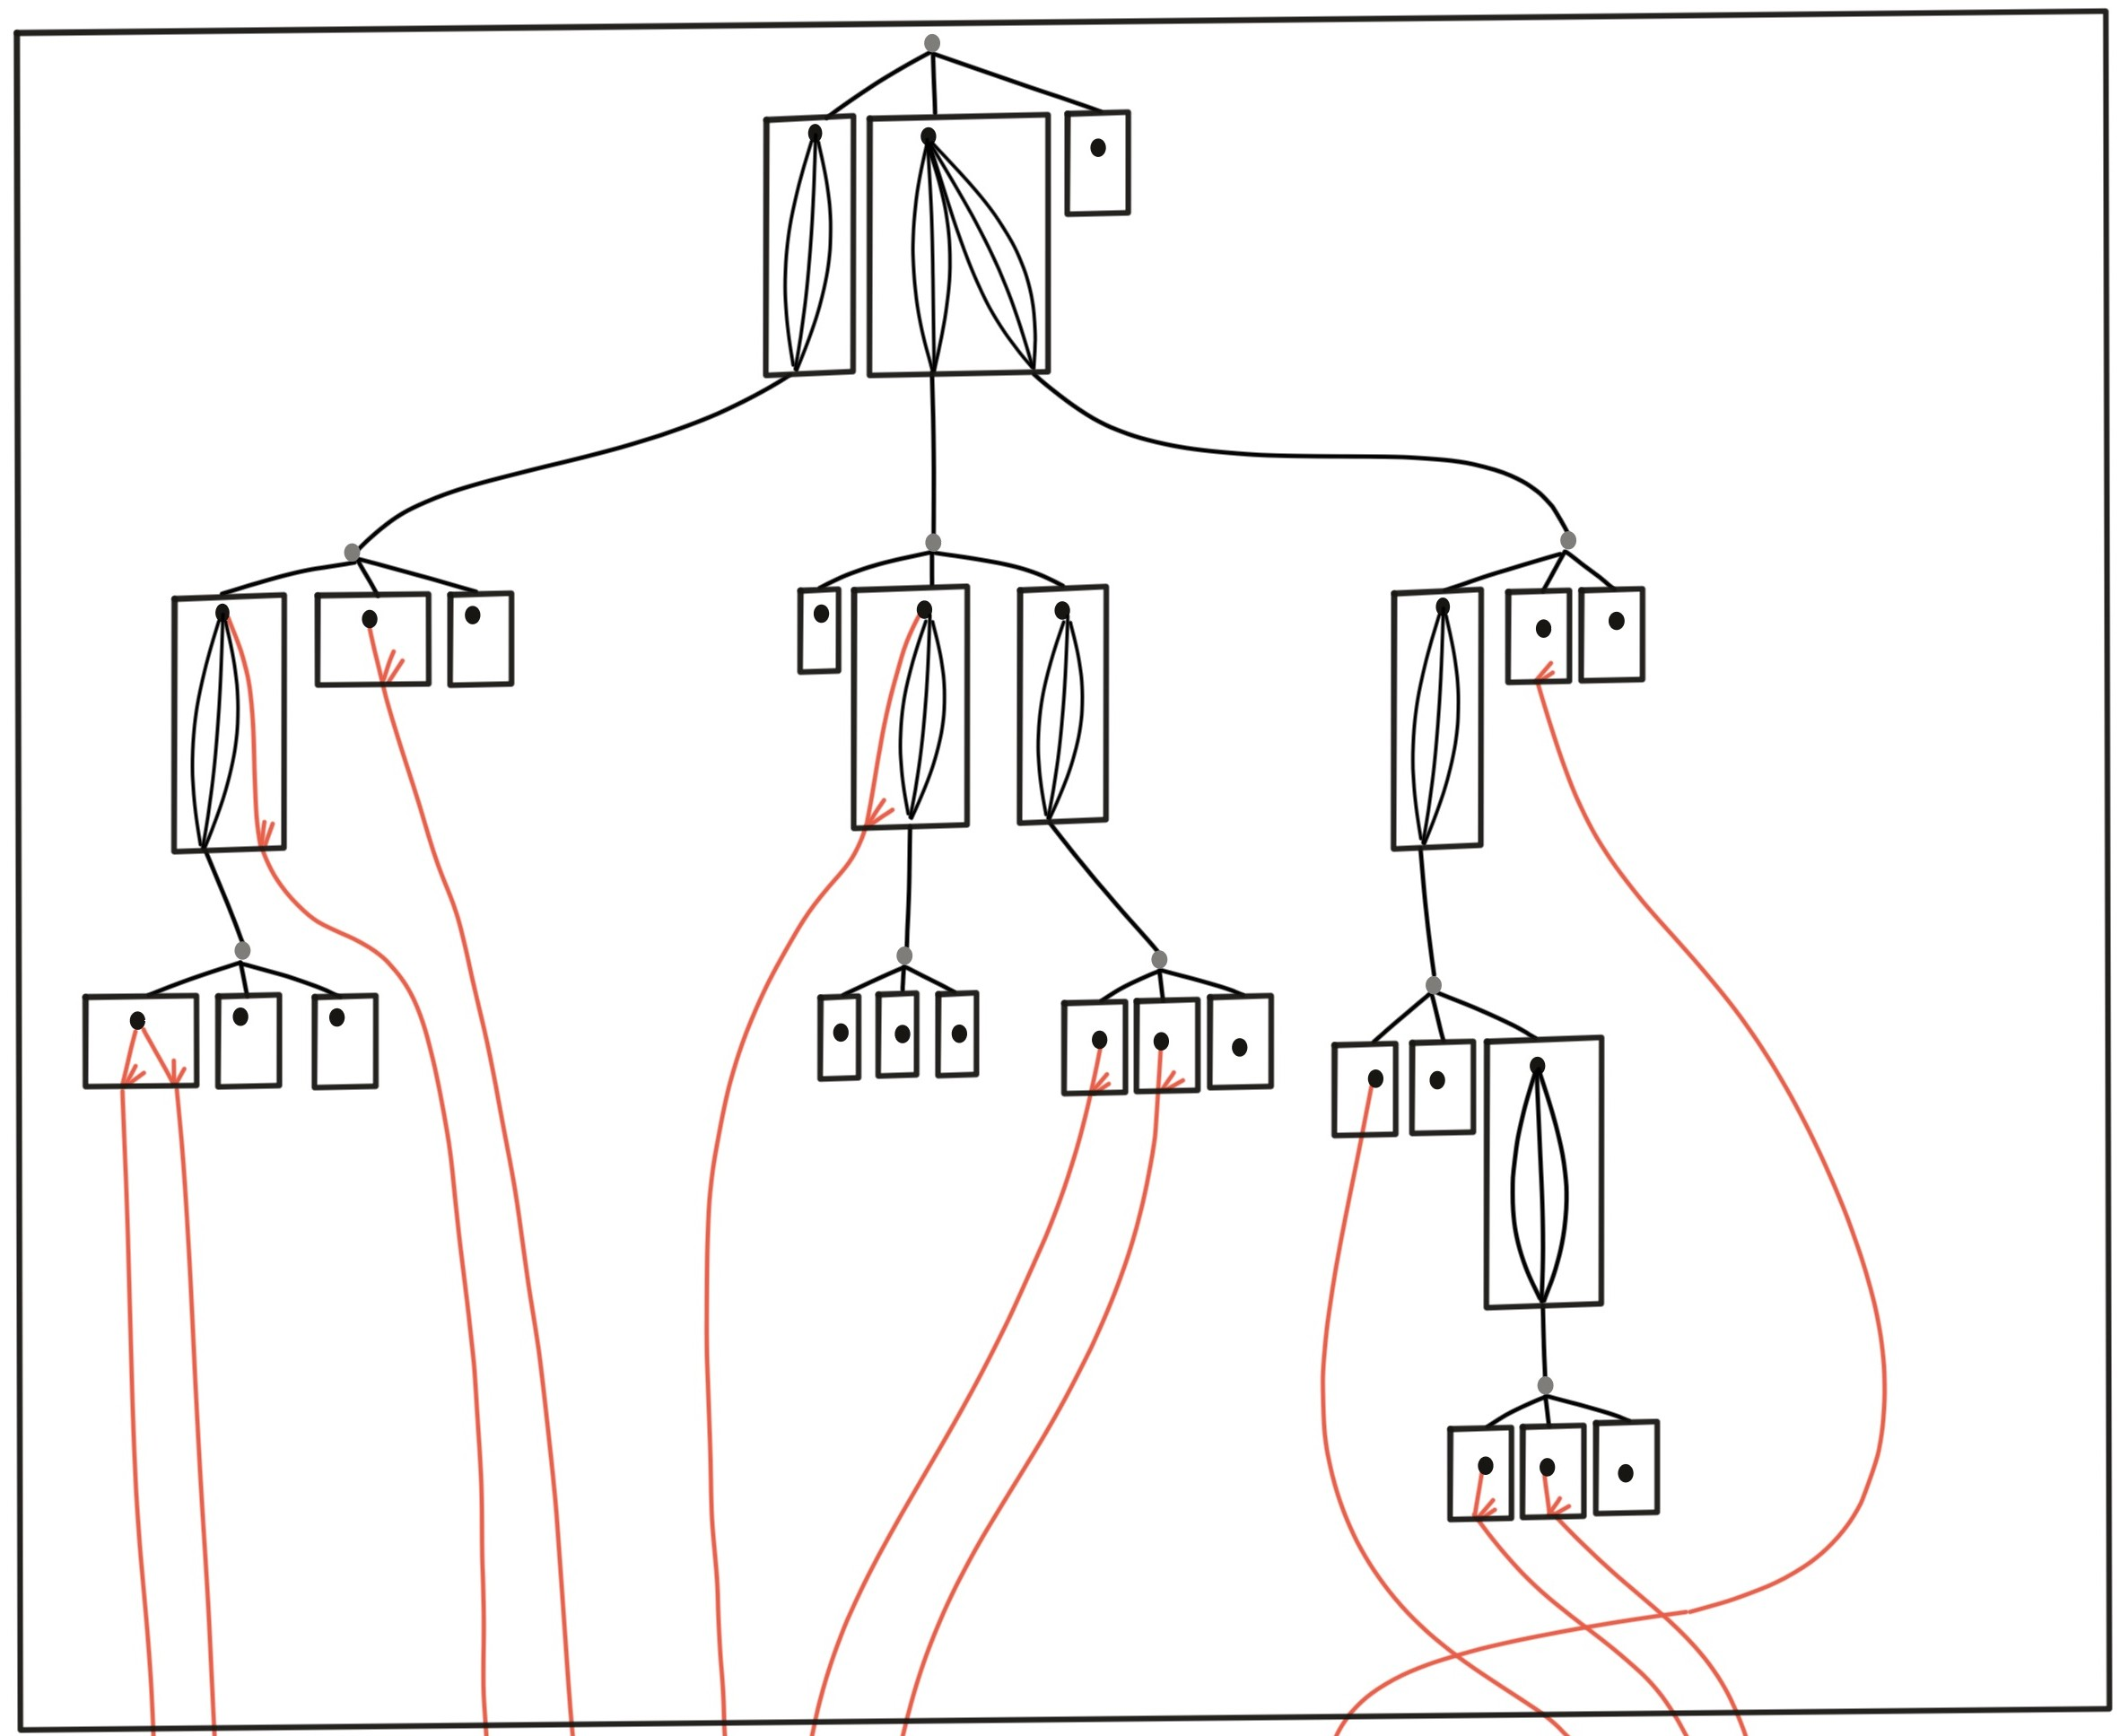
\includegraphics[scale=.07]{MyPic36.jpg}
\end{center} 
\begin{center}
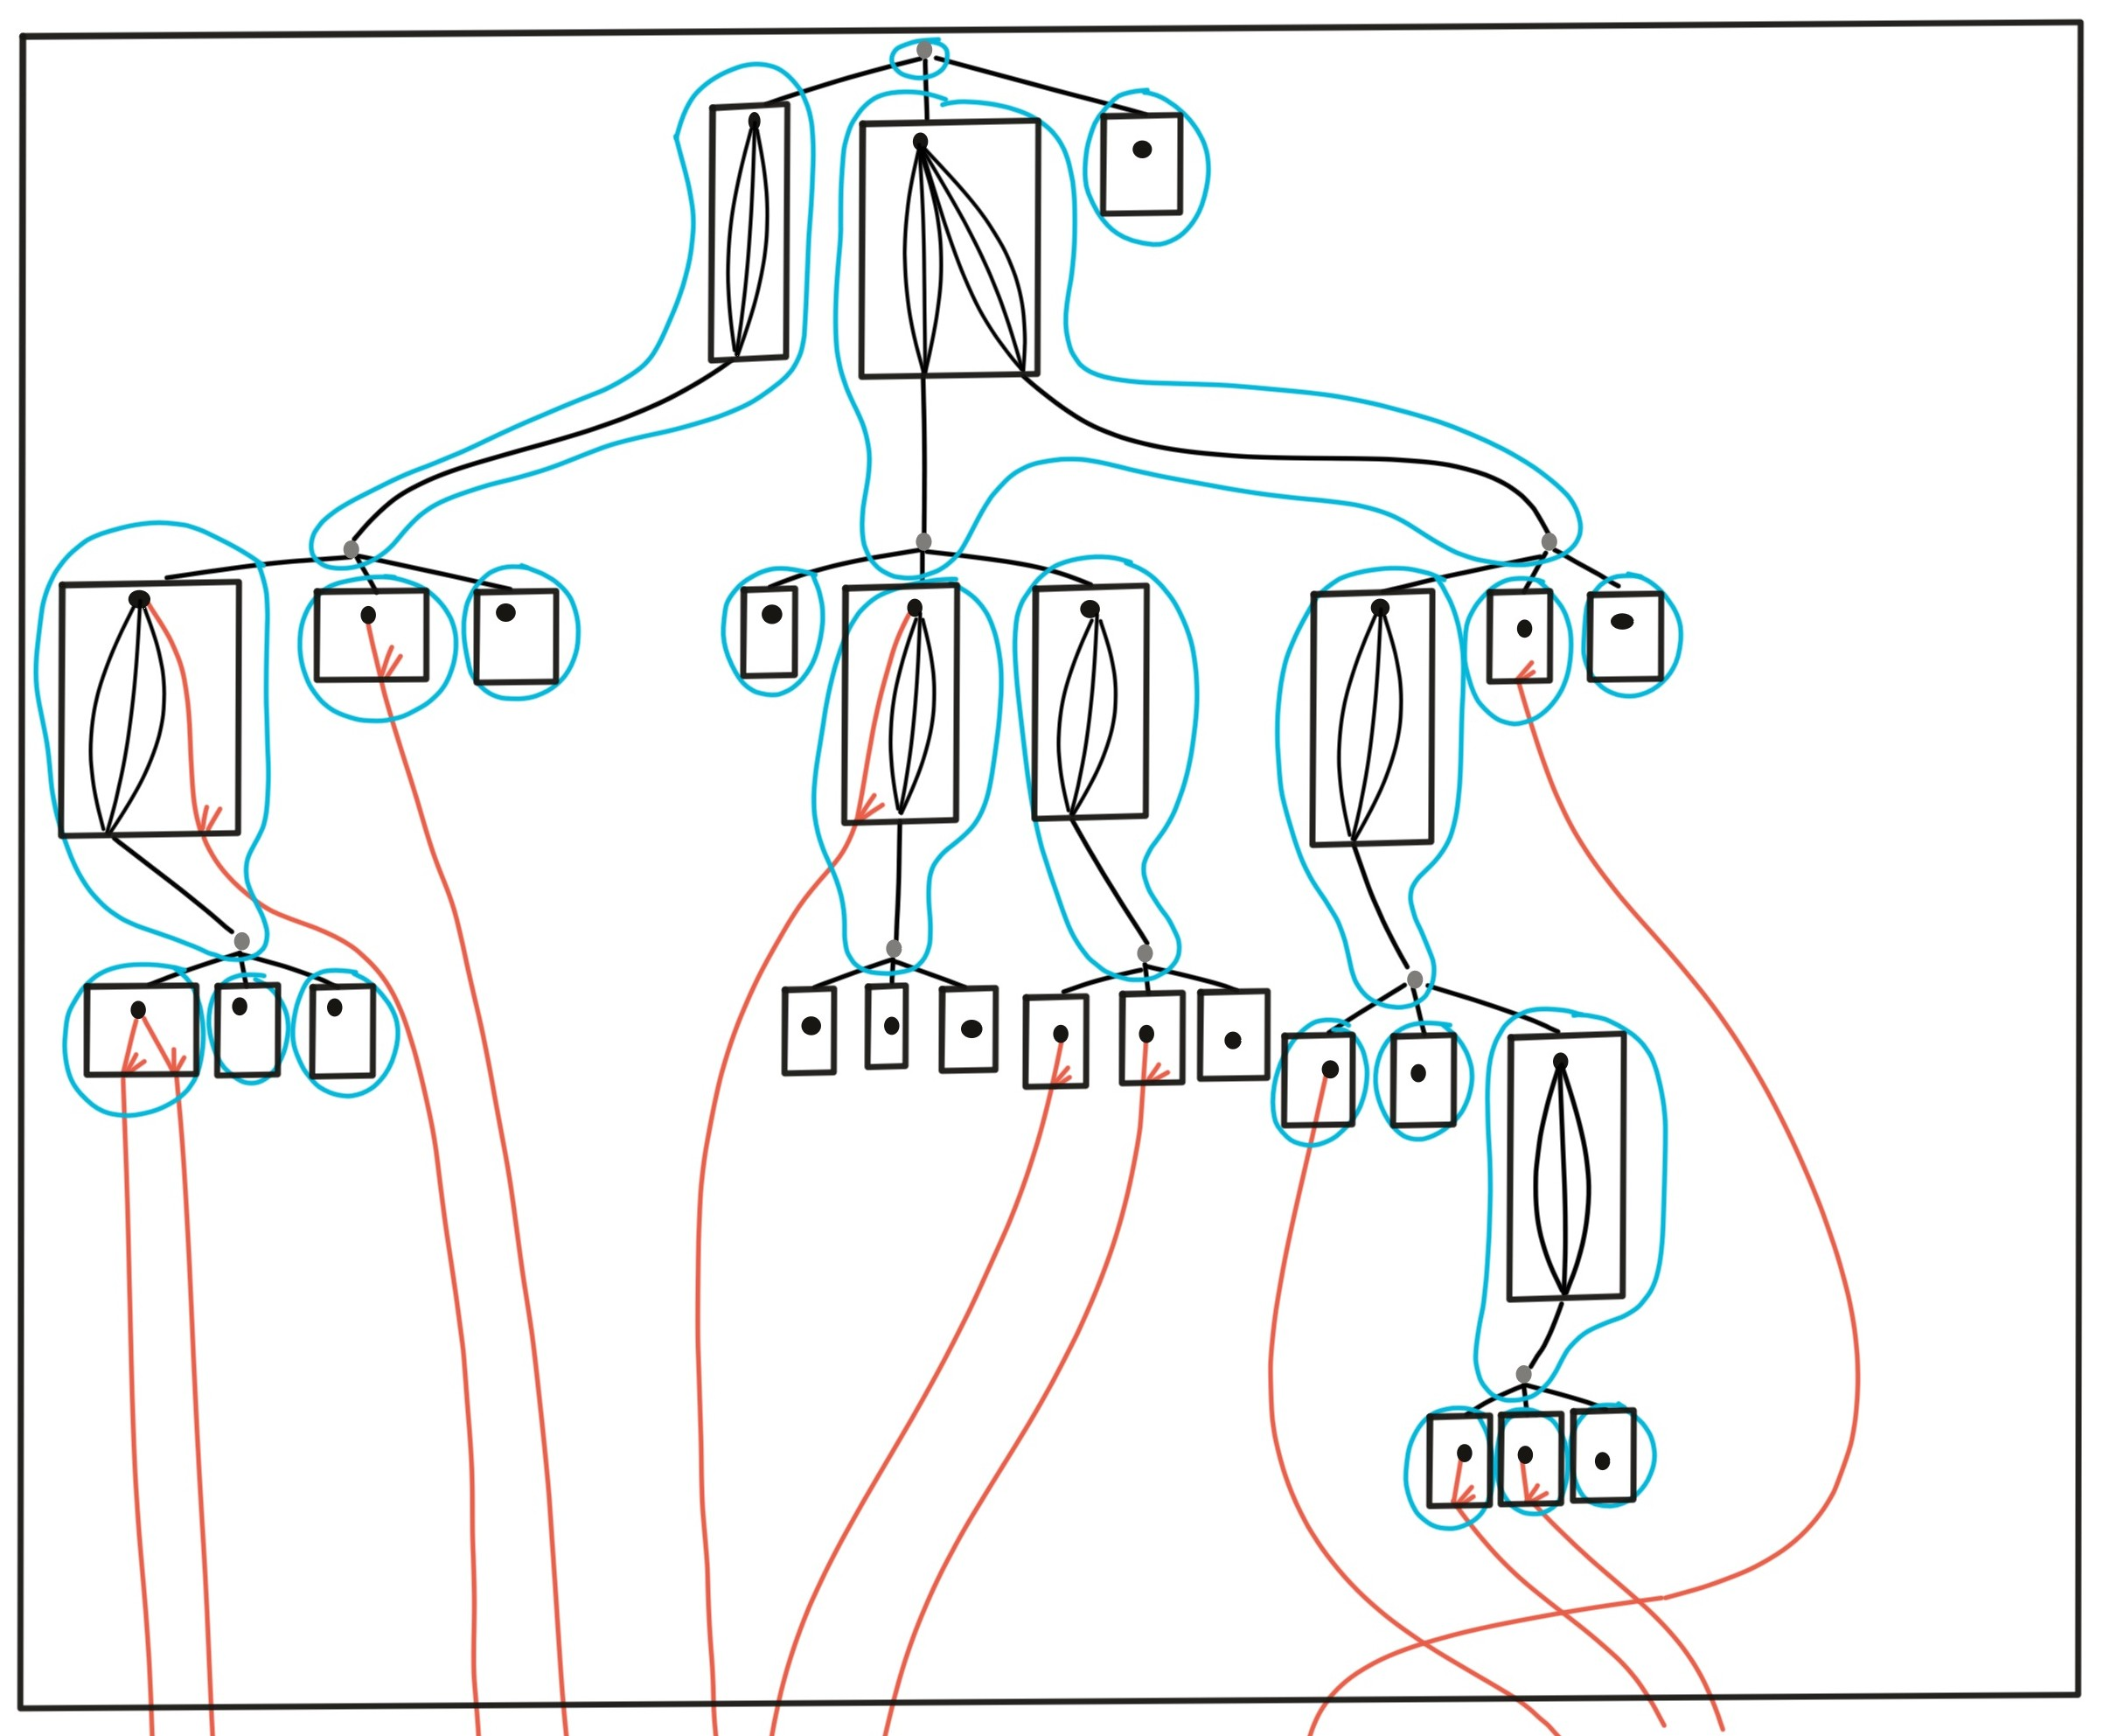
\includegraphics[scale=.07]{MyPic37.jpg}
\end{center} 
\begin{center}
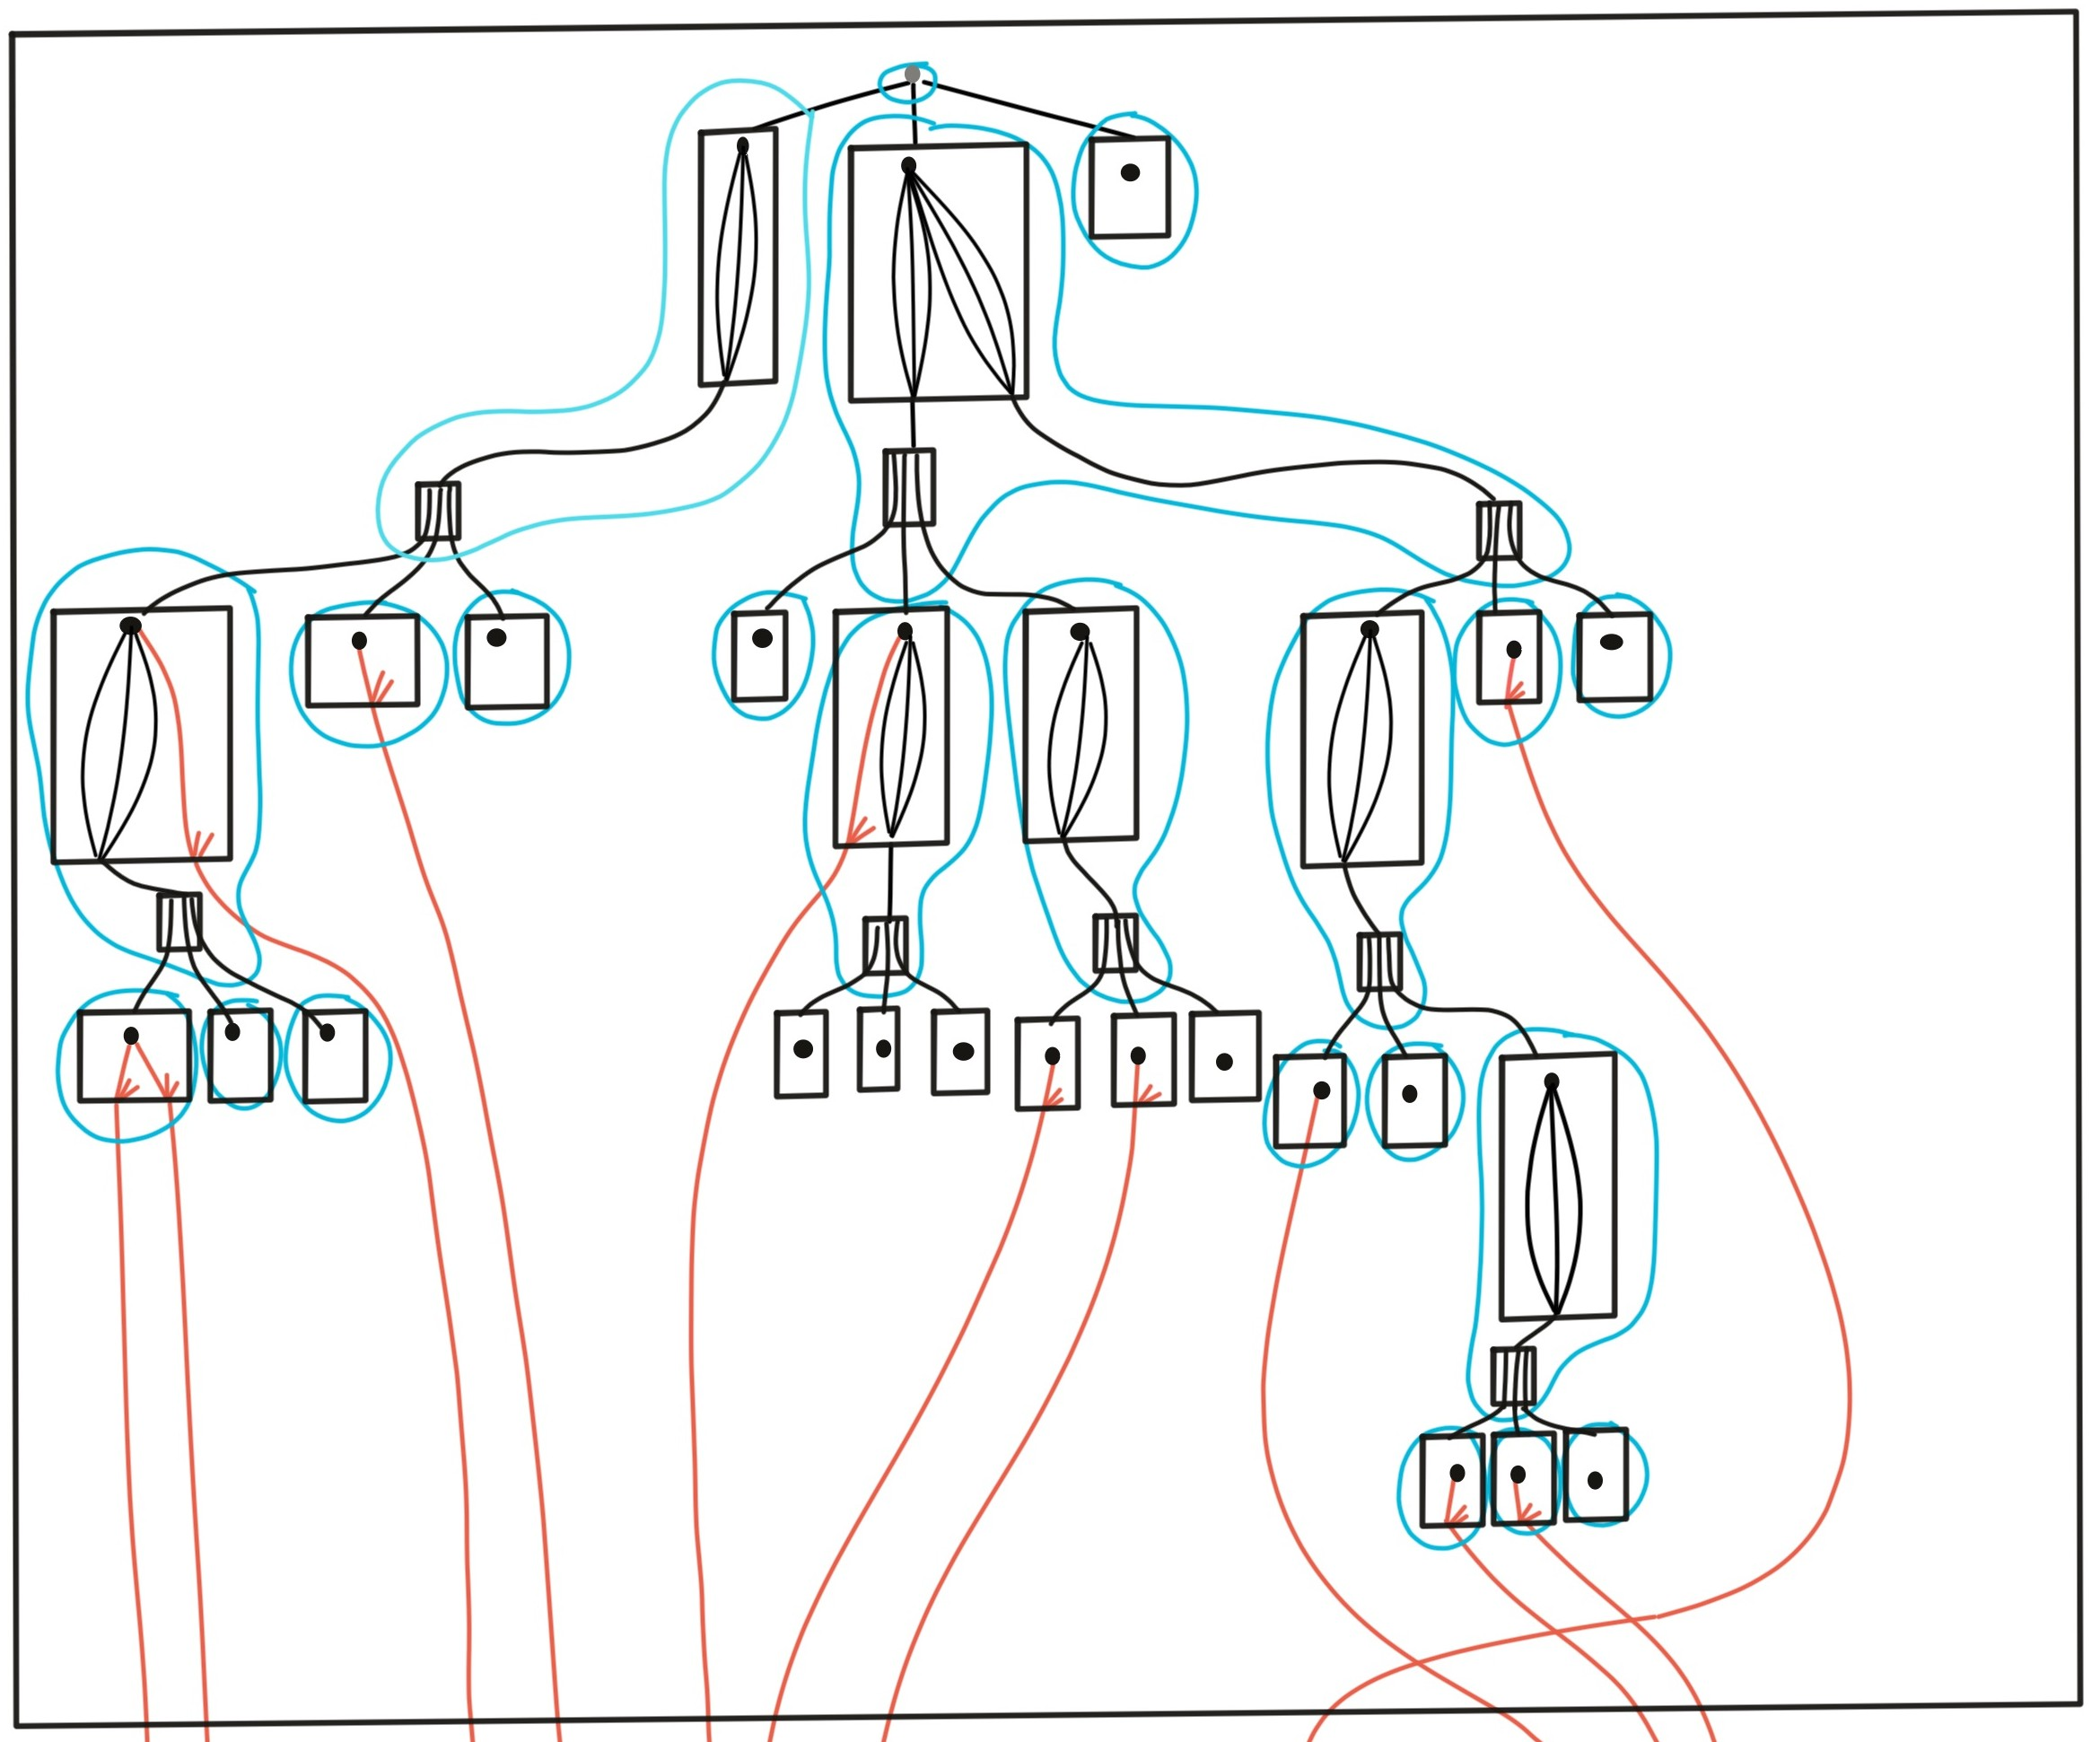
\includegraphics[scale=.07]{MyPic38.jpg}
\end{center} 
\begin{center}
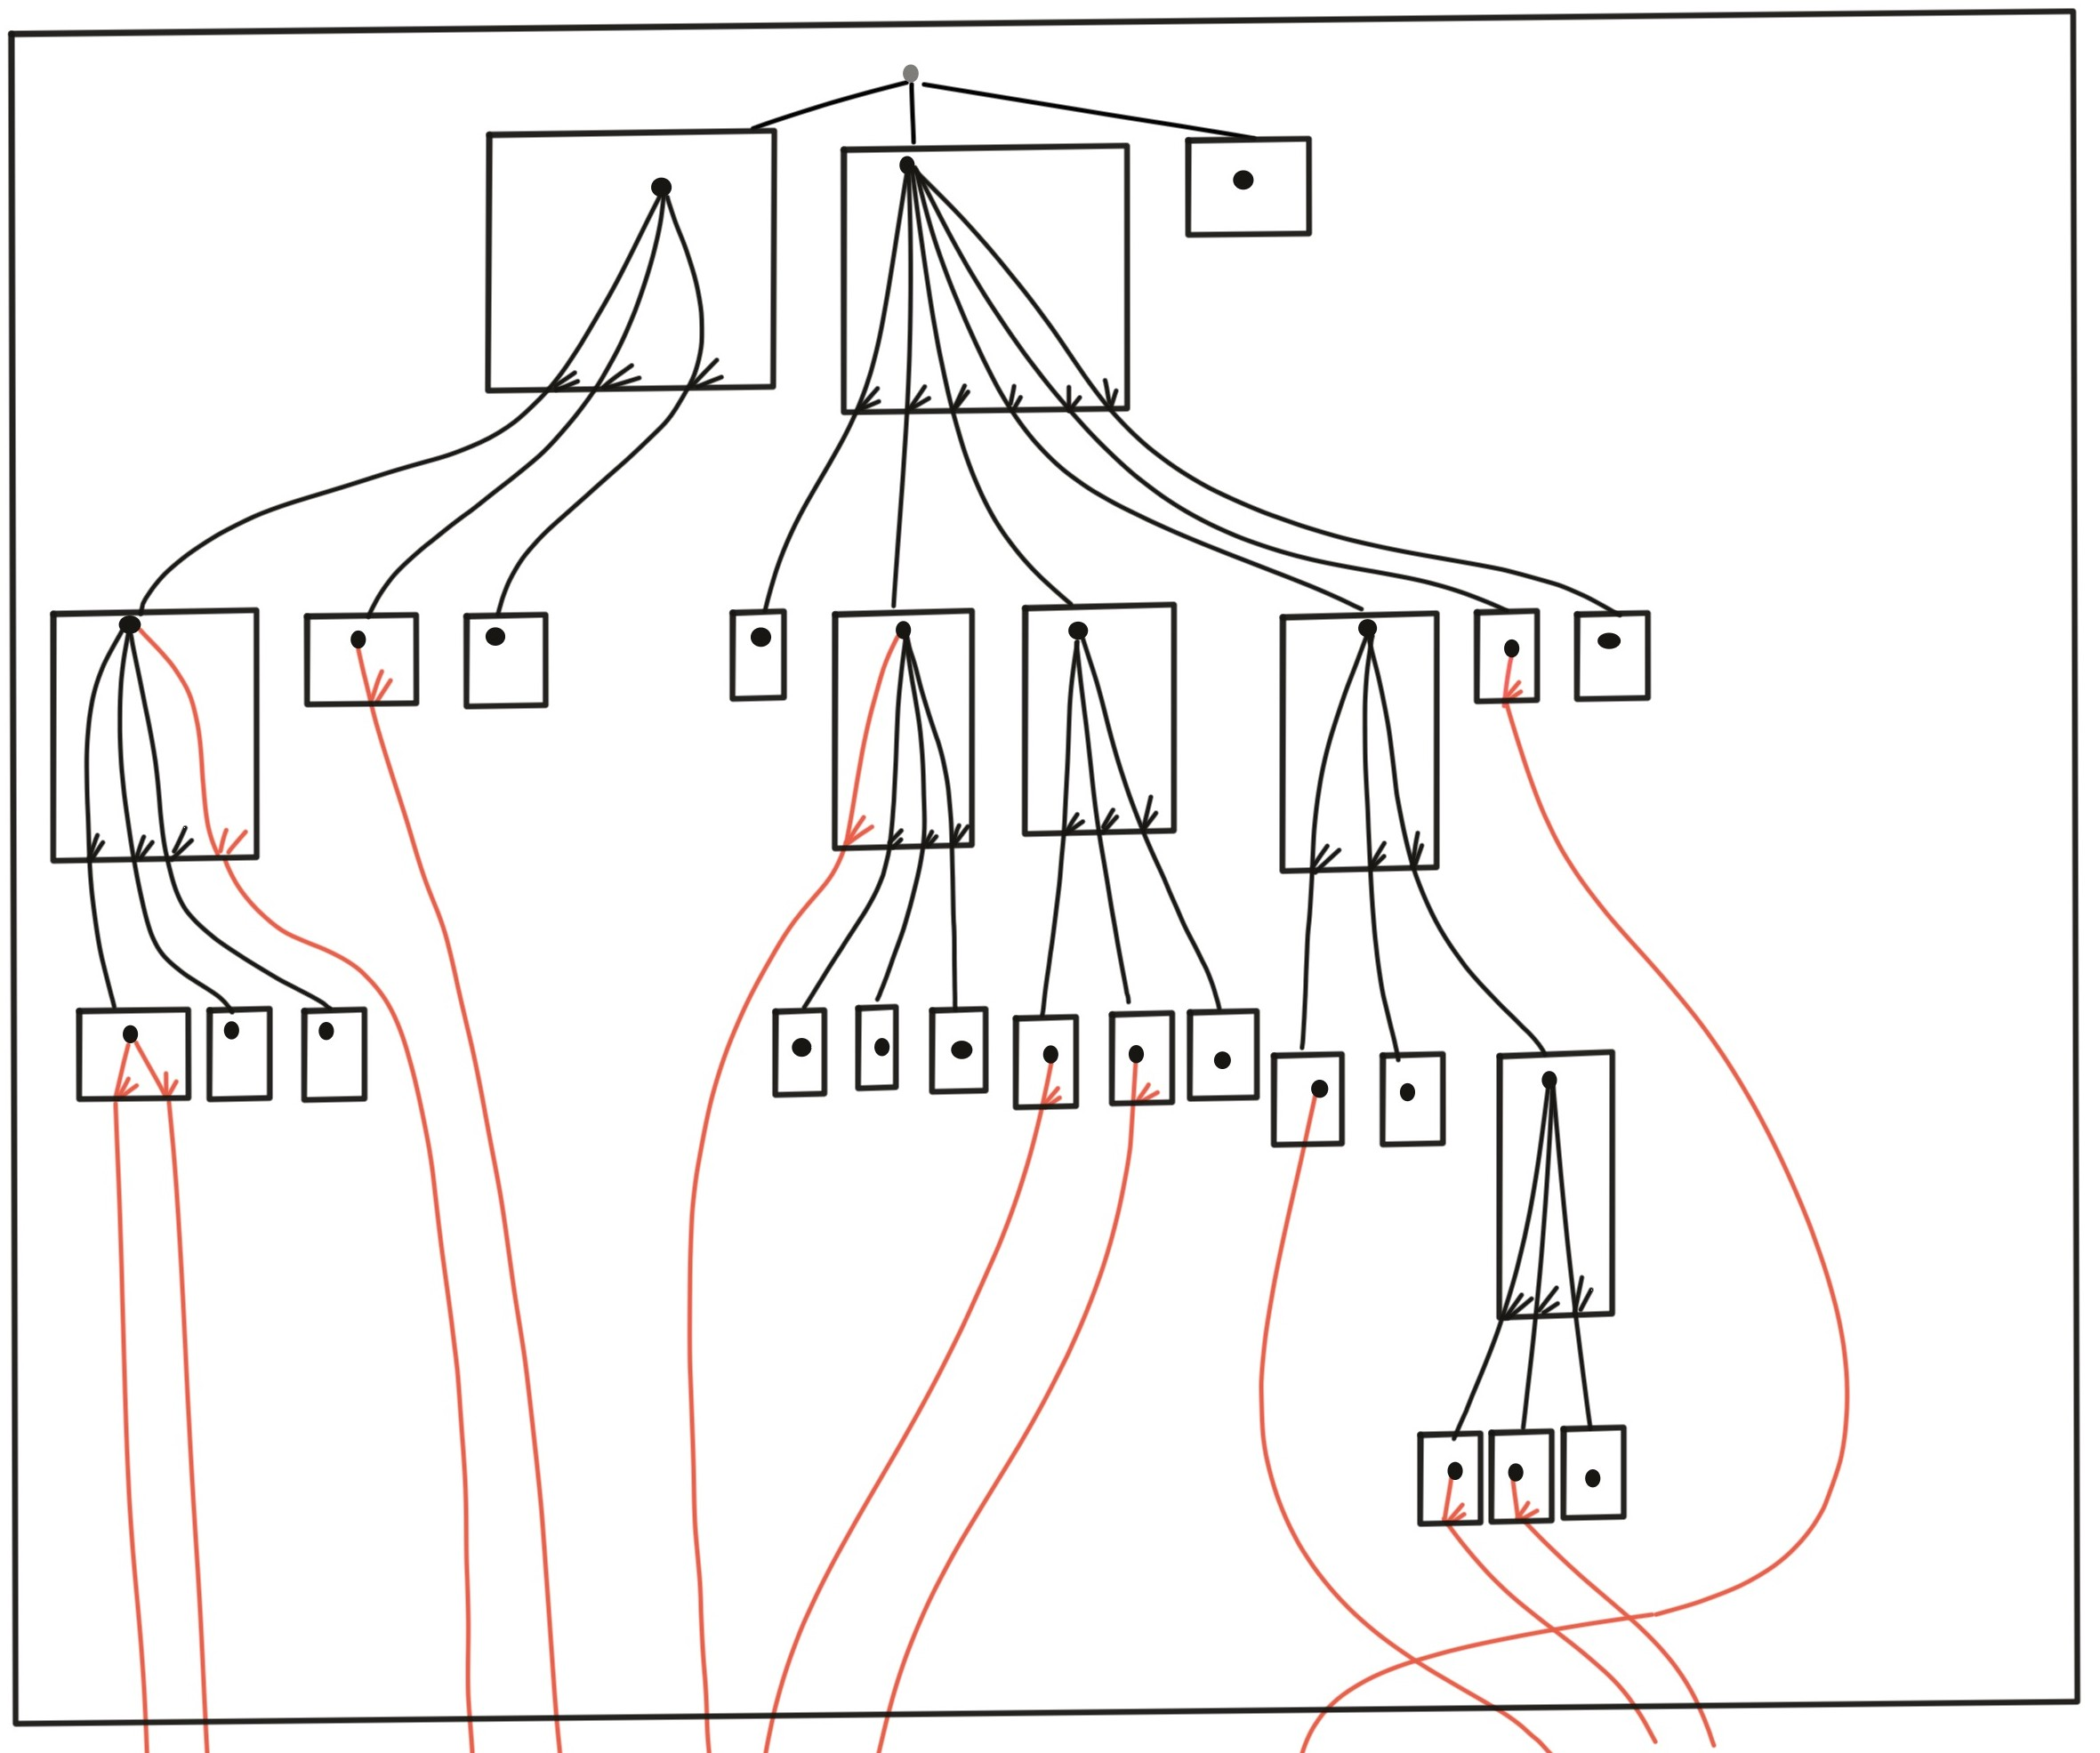
\includegraphics[scale=.07]{MyPic39.jpg}
\end{center} 
\end{proof}
